%
% The standard LaTeX article class is close to what is needed for an MPhys project report
\documentclass[12pt]{article}

% The following package makes the necessary tweaks to comply with the formatting requirements.
% It also provides a standardised title page, and will warn you if the main text is too long.
\usepackage{mphysproject}
%
%% DO NOT GO CHANGING THE FONT SIZE OR MARGINS! If your main text doesn't fit within 50 pages,
%% you will have to cut stuff out.
%
%% REMEMBER: The target length is around 35 pages
%

% The formatting of the document can be enhanced by loading extra packages.
%
% An essential package is `graphicx', which is loaded by the mphysproject package so you don't
% need to load this yourself. This allows you to include figures using the \includegraphics command.
% To get more information about a package, type texdoc <package> on the Unix command line,
% substituting <package> with the name of the package, e.g., texdoc graphicx
%
% For a wider variety of mathematical environments, symbols and formatting options:
%\usepackage{amsmath,amssymb}
%
% If you want to use colour in the text
%\usepackage{color}
%
% If you want to put figures side by side with separate captions
%\usepackage{subfigure}
% For sub figures, subfigure package is depreciated.
\usepackage{subcaption}
% If you happen to dislike the standard TeX fonts
%\usepackage{times}
%
% If you include any URLs in your text and/or want to make cross-references clickable, include one of the following
% two lines
\usepackage{hyperref}  % This enables hyperlinks but leaves them in black, which is best for printing
%\usepackage[colorlinks=true]{hyperref} % This colours the hyperlinks, which is better for screen reading
% For Bra-Ket notation.
\usepackage{braket}
% For pictures.
\usepackage{tikz}
% For creating data plots.
\usepackage{pgfplots}
\pgfplotsset{compat=1.12}
% For maths symbols.
\usepackage{amsfonts}
% For colon equals.
\usepackage{mathtools}
% For adding todo notes.
\usepackage[textsize=tiny]{todonotes}
% For nice bold vector symbols.
\usepackage{bm}
% For nicer fractions.
\usepackage[nice]{nicefrac}
% For Tiny font size.
\usepackage{lmodern}
% For more floats
\usepackage{morefloats}

\begin{document}

\title{Accelerated Tempering Dynamics in HMC Simulations of Lattice Field Theory} % Place your project title in here
\author{Jack Frankland} % Put your name here
\supervisor{Dr Roger Horsley} % Place your principal supervisor here
\supervisor{Dr Brian Pendleton} % If you have additional supervisors, list them with separate \supervisor commands
%\date{1st January 2018} % Today's date will appear on the title page by default, but if you want to tie this to a particular date, you can do so here

% Insert your abstract below
\begin{abstract}
    
\end{abstract}

% This command is essential to make the title page appear
\maketitle

% This command introduces the Personal Statement
\personalstatement



% If you have anyone that needs to be acknowledged (e.g., anyone who provided assistance with your project work,
% provided data etc) please do so here. Delete this (or comment it out) if you have no-one to acknowledge.
\acknowledgments
I wish to extend my deep appreciation and gratitude to Dr. Roger Horsely and Dr. Brian Pendleton, my MPhys project supervisors, for all their guidance in answering questions as well as providing feedback, advice, support and encouragement throughout the entire project, both in our weekly meetings and through electronic communications.



% This command inserts a table of contents, and sets things up for the main text of your report.
% The page count starts from here. DO NOT DELETE OR DISABLE THIS COMMAND!
\maintext
\section{Introduction}
 The Hybrid Monte Carlo (HMC) algorithm (also referred to as Hamiltonian Monte Carlo) was originally developed by Duane, Kennedy, Pendleton and Roweth in \cite{duane_kennedy_pendleton_roweth_1987} for the purposes of numerical simulation of lattice field theory. HMC is an example of a Markov Chain Monte Carlo (MCMC) method where states are proposed via a Markov chain in order to produce samples distributed according to some probability distribution, these samples can then be used to estimate the expectation value of some function of the samples under the probability distribution. Although MCMC was original introduced via the \textit{Metropolis algorithm} in \cite{metropolis_rosenbluth_rosenbluth_teller_teller_1953}, HMC makes improvements on this method by using Hamiltonian dynamics to propose new states in the Markov chain. The idea is that we consider the variables of interest as \textit{position} and introduce auxiliary \textit{momentum} variables which we can use to define a Hamiltonian and evolve the system in computer time via a leapfrog integration method to propose new states. We alternate between drawing the momentum variables from a multivariate Gaussian distribution and performing a Metropolis update where the new state state is proposed via the Hamiltonian dynamics. The advantage of the HMC method is that the proposed state can have a high probability of acceptance and be distant from the current state, it therefore avoids the problems of slow state exploration that results from using random-walk proposals such as in the original Metropolis algorithm \cite{neal_2011}. Although popular amongst the lattice field theory community the HMC method has also been used in statistics, e.g. \cite{neal_1996_a}, \cite{ishwaran_1999} and \cite{schmidt_2009} for applications such as neural network models. However, our application of HMC will be to quantum mechanical systems and in particular the case of quantum harmonic and anharmonic oscillators.

 Standard HMC can have difficulty sampling from the different areas of a probability distribution if those areas are separated by a region of low probability; we will refer to these areas as \textit{isolated modes} of the distribution. An example of this in quantum mechanics is that of a 1-dimensional double well potential, where the probability of finding a particle in either well is high, whilst finding it in the region between the wells is low. If we are interested in generating samples for say the position of the particle using the HMC algorithm, then for a deep enough well there will be an asymmetry in the number of samples recorded in each well. This is due to the energy cost associated with moving between the wells, and so the Hamiltonian dynamics in the HMC simulation will tend to propose an update state in the well the current state is in, leading to the asymmetry in the recorded samples. The aim of this project is to write an HMC simulation of the anharmonic oscillator and introduce a tempering parameter as proposed in \cite{neal_2011} and \cite{neal_1996_b} into the dynamics to investigate whether this increases the frequency at which samples move between the two wells. In terms of our simulation the benefit of successful tempering would be more accurate estimations of observed quantities such as position expectation and ground state density functions. However, in terms of a broader goal, successful tempering results in HMC simulations of simple quantum mechanical systems, may suggest it has potential applications in lattice field theory where isolated modes are a more serious problem. In certain field theories, including QCD, the states we wish to construct via our Markov chain are in ``distinct topological sectors which are labelled by a topological charge''\cite{bietenholz_2016}. For small lattice spacings moving between these sectors can take a very long time, since they are separated by a region of high Euclidean action (i.e. low probability in the distribution) and so the transitions are statistically suppressed \cite{bietenholz_2016}, \cite{debbio_panagopoulos_vicari_2002} and \cite{debbio_manca_vicari_2004}. It is therefore possible that tempered dynamics will have applications to theories such as lattice QCD where isolated modes arise as regions of distinct topological charge. In general the \textit{autocorrelation time} which measures how correlated subsequent samples in any Monte Carlo simulation are will be high if the system is trapped in an isolated mode. The purpose of tempering is to try and diminish the autocorrelation time without the need for extra computation. 

 In this report we follow the work of Creutz and Freedman in \cite{creutz_freedman_1981} who constructed a MCMC simulation of the harmonic and anharmonic oscillators, however we will use HMC where they used the Metropolis algorithm. Reproducing the results in \cite{creutz_freedman_1981} using the Metropolis algorithm is a popular choice for undergraduate projects e.g. \cite{westbroek_king_vvedensky_durr_2017}, \cite{rodgers_raes} and \cite{slapik_serenone} which provide a useful comparison for our simulation which uses a different algorithm. We begin the report by following the steps taken in \cite{creutz_freedman_1981} where we introduce and define the path integral of quantum mechanics and show that for a discrete lattice in Euclidean time the path integral can be considered as a canonical partition function. This connection between quantum mechanics and statistical physics is what will enable us to apply Monte Carlo methods and we will see that the quantum expectation values in the ground state correspond to classical expectation values of the statistical system with a canonical distribution. We will then briefly review the topic of Monte Carlo methods and explain how they can be used to approximate expectation values for functions of random variables under some probability distribution via a Markov chain as well as defining detailed balance and ergodicity which are conditions required for the Monte Carlo simulation to be valid. Before introducing the HMC algorithm we very briefly review Hamiltonian dynamics, explain how Hamilton's equations can be integrated numerically via the leapfrog method and show that as well as being reversible, the leapfrog method preserves volume on the phase space of position and momentum coordinates, which we we will see is necessary for detailed balance to hold. Having provided the relevant background we are then able to define the steps of the HMC algorithm and explain how it can be used to sample from a canonical distribution by defining axillary momenta coordinates and a Hamiltonian. In this section we will also discuss the issue of ergodicity and show that HMC obeys detailed balance. Due to the stochastic nature of MCMC algorithms, samples in the Markov chain can be correlated and we briefly discuss the effect of this on data analysis. The results section begins by applying the HMC algorithm to the canonical distribution for the quantum system. We examine the results of our simulation for the harmonic oscillator where we are able to compare with numerical and exact results for the discrete theory in \cite{creutz_freedman_1981},\cite{westbroek_king_vvedensky_durr_2017}, \cite{rodgers_raes} and \cite{slapik_serenone}. The simple system of the harmonic oscillator provides a good testing ground for our simulation where we can easily compare our results to theory. Moving on to the anharmonic oscillator we are able to apply our simulation to a system that does not have an analytic solution. For the case of the anharmonic oscillator we are able to compare our results to those acquired through alternative methods \cite{blankenbecler_degrand_sugar_1980} and simulations \cite{rodgers_raes} however we will observe in this section that the HMC simulation begins to fail in the case of the isolated modes in the double well potential. In particular the double well system can have difficulty tunnelling between the two modes. At this point we will examine the effects of introducing a tempering parameter into the simulation, with the hope that it will increase the tunnel rate. We will show that volume preservation still holds for tempered dynamics, which is necessary if it is still to obey detailed balance.


\section{Background}
    \subsection{Quantum Mechanics}
        \subsubsection{The Path Integral}
        \label{sec:QuantumMechanics}
        In quantum mechanics we are often interested in calculating the path integral:
        \begin{equation}
            \label{eq:PathIntegral}
            \braket{x_b,t_b|x_a,t_a} = \int_{x_a}^{x_b} {\cal D} x\left(t\right) \exp{\left(\frac{i}{\hbar} S_M\left[x\left(t\right)\right]\right)},
        \end{equation}
        where we will use the notation:
        \begin{align}
            \label{eq:PathIntegralZ_fi}
            Z_{ba} & = \braket{x_b,t_b|x_a,t_a} \\
            \label{eq:PathIntegralZ_fi2}
                   & = \bra{x_b}e^{-i\left(t_b-t_a\right)\hat{H}/\hbar}\ket{x_a},
        \end{align}
        where $\hat{H}$ is the usual quantum mechanical Hamiltonian operator:
        \begin{equation}
            \hat{H}\left(\hat{p},\hat{x}\right) = \frac{\hat{p}^2}{2m} + \hat{V}\left(\hat{x}\right).
        \end{equation} 
        $Z_{ba}$ is the transition amplitude for a particle of mass $m$ in position eigenstate (in the Heisenberg picture) $\ket{x_a,t_a}$ to move to position eigenstate $\ket{x_b,t_b}$; this gives us the probability amplitude of a particle at $x_a$ at time $t_a$ to move to position $x_b$ at time $t_b$. The term on the right of equation \ref{eq:PathIntegral} is known as the \textit{Feynman path integral}. The measure $\int {\cal D} x\left(t\right)$ is an integral over all paths between $x_a$ and $x_b$ and $S_M\left[x\left(t\right)\right]$ is the Minkowski action of a particle of mass $m$ on the path $x\left(t\right)$ which is defined by:
        \begin{equation}
            \label{eq:MinkowskiAction}
            S_M\left[x\left(t\right)\right] = \int_{t_a}^{t_b} dt \left[\frac{1}{2}m\left(\frac{dx}{dt}\right)^2 - V(x)\right],
        \end{equation}
        where $x\left(t_a\right) = x_a$ and $x\left(t_b\right) = x_b$ are the boundary conditions, and $V\left(x\right)$ (now a function) is the potential the particle is in.

        Due to the oscillating integrand in equation \ref{eq:PathIntegral}, it is not clear the integral will converge, and the integral measure needs to be defined before we proceed. In order to do this we follow the steps taken by Creutz and Freedman in \cite{creutz_freedman_1981} to get equation \ref{eq:PathIntegral} into a form we can work with.



        \begin{figure}
            \centering
            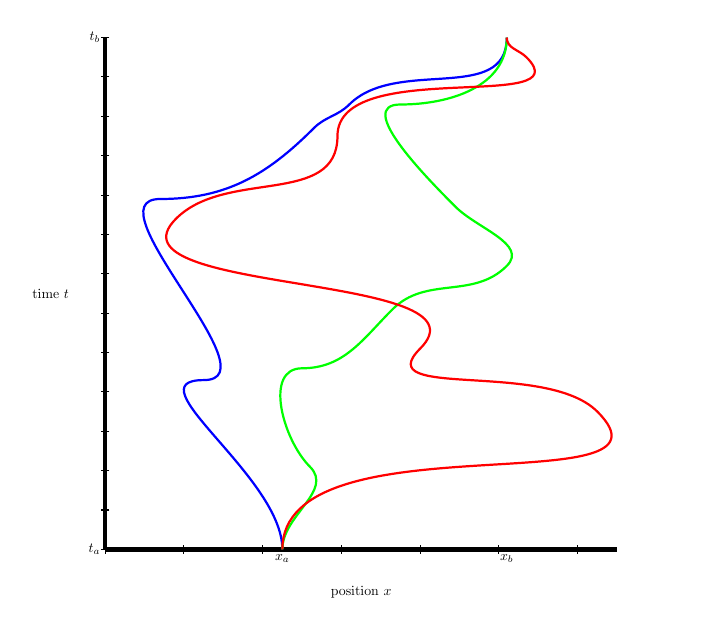
\begin{tikzpicture}[scale=0.5, every node/.style={transform shape}]
                \draw [ultra thick] [-] (0,13) -- coordinate (y axis mid) (0,0);
                \draw [ultra thick] [-] (0,0) -- coordinate (x axis mid) (13,0);
                \foreach \x in {0,2,...,13}
                    \draw (\x,3pt) -- (\x,-3pt);
                \foreach \y in {0,...,13}
                    \draw (3pt,\y) -- (-3pt,\y);
                \node[below=0.8cm] at (x axis mid) {position $x$};
                \node[left=0.8cm] at (y axis mid) {time $t$};
                \node [left] at (0,0) {$t_{a}$};
                \node [left] at (0,13) {$t_{b}$};
                \node [below] at (4.5,0) {$x_a$};
                \node [below] at (10.2,0) {$x_b$};
                \draw [-,thick, blue] (4.5,0) to [out=90,in=180] (2.5,4.3)
                        to [out=0,in=180] (1.4,8.9) to [out=0,in=-135] (5.3,10.7) 
                        to [out=45,in=225] (6.2,11.3) to [out=45,in=-90] (10.2,13);
                \draw [-,thick, green] (4.5,0) to [out=90,in=-45] (5.2,2.1)
                        to [out=135,in=180] (5.0,4.6) to [out=0,in=-135] (7.3,6.1) 
                        to [out=45,in=225] (10.2,7.2) to [out=45,in=-45] (8.9,8.7)
                        to [out=135,in=180] (7.5,11.3) to [out=0,in=-90] (10.2,13);
                \draw [-,thick, red] (4.5,0) to [out=90,in=-45] (12.5,3.5)
                        to [out=135,in=225] (8,5.1) to [out=45,in=-135] (1.8,8.4) 
                        to [out=45,in=270] (5.9,10.5) to [out=90,in=-45] (10.7,12.5)
                        to [out=135,in=-90] (10.2,13);
            \end{tikzpicture}
            \caption{Three of the infinitely many paths from $\left(x_a,t_a\right)$ to $\left(x_b,t_b\right)$ that contribute to the path integral.} 
            \label{fig:ExamplePathIntegrals}
        \end{figure}
        \subsubsection{Connecting to Statistical Physics}
        In the transition amplitude we integrate over an infinite number of paths, figure \ref{fig:ExamplePathIntegrals} shows three such paths that contribute to the path integral. The first step in calculating the path integral is to discretise time, this is shown in figure \ref{fig:TimeLattice} where we have discretised the \textcolor{green}{green} path in figure \ref{fig:ExamplePathIntegrals} onto a time lattice and we assume the particle travels along a straight line between the time sites.
        \begin{figure}
            \centering
            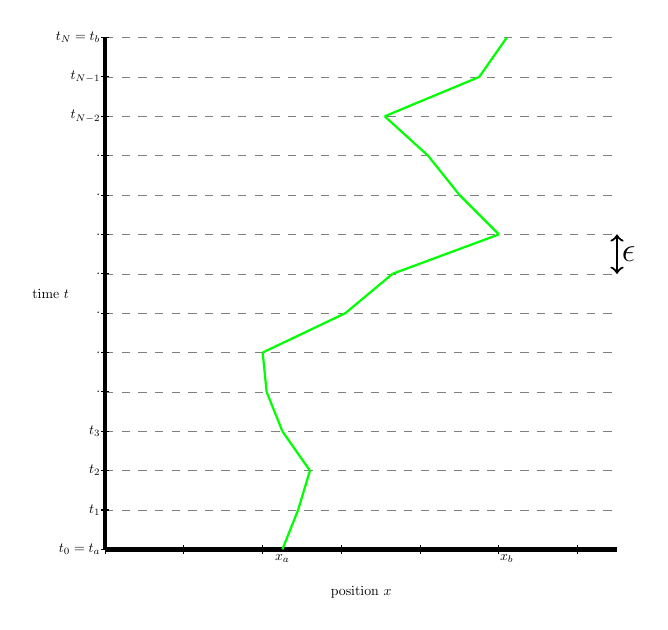
\begin{tikzpicture}[scale=0.5, every node/.style={transform shape}]
                
                \foreach \y in {0,...,13}{ \draw [help lines, dashed] (0,\y) -- (13,\y); }
                \draw [ultra thick] [-] (0,13) -- coordinate (y axis mid) (0,0);
                \draw [ultra thick] [-] (0,0) -- coordinate (x axis mid) (13,0);
                \foreach \x in {0,2,...,13}
                    \draw (\x,3pt) -- (\x,-3pt);
                \foreach \y in {0,...,13}
                    \draw (3pt,\y) -- (-3pt,\y);
                \node [left] at (0,0) {$t_{0}=t_{a}$};
                \node [left] at (0,1) {$t_{1}$};
                \node [left] at (0,2) {$t_{2}$};
                \node [left] at (0,3) {$t_{3}$};
                \node [left] at (0,4) {$.$};
                \node [left] at (0,5) {$.$};
                \node [left] at (0,6) {$.$};
                \node [left] at (0,7) {$.$};
                \node [left] at (0,8) {$.$};
                \node [left] at (0,9) {$.$};
                \node [left] at (0,10) {$.$};
                \node [left] at (0,11) {$t_{N-2}$};
                \node [left] at (0,12) {$t_{N-1}$};
                \node [left] at (0,13) {$t_{N}=t_{b}$};
                \node[below=0.8cm] at (x axis mid) {position $x$};
                \node[left=0.8cm] at (y axis mid) {time $t$};
                \draw [thick] [<->] (13,7) -- (13,8) ;
                \node [below=0.5cm,font=\fontsize{30}{0}] [right] at (13,8) {$\epsilon$};
                \draw [thick,green] (4.5,0) -- (4.9,1);
                \draw [thick,green] (4.9,1) -- (5.2,2);
                \draw [thick,green] (5.2,2) -- (4.5,3);
                \draw [thick,green] (4.5,3) -- (4.1,4);
                \draw [thick,green] (4.1,4) -- (4.0,5);
                \draw [thick,green] (4.0,5) -- (6.1,6);
                \draw [thick,green] (6.1,6) -- (7.3,7);
                \draw [thick,green] (7.3,7) -- (10,8);
                \draw [thick,green] (10,8) -- (9.0,9);
                \draw [thick,green] (9.0,9) -- (8.2,10);
                \draw [thick,green] (8.2,10) -- (7.1,11);
                \draw [thick,green] (7.1,11) -- (9.5,12);
                \draw [thick,green] (9.5,12) -- (10.2,13);
                \node [below] at (4.5,0) {$x_a$};
                \node [below] at (10.2,0) {$x_b$};
            \end{tikzpicture}
            \caption{Discretising time and a path from $\left(x_a,t_a\right)$ to $\left(x_b,t_b\right)$  onto a lattice of time spacing $\epsilon$.}
            \label{fig:TimeLattice}
        \end{figure}
        For each time site $t_i$ on the lattice we have a continuous position variable $x_i = x\left(t_i\right)$ where $i=0,1,\dots,N$ which gives the position of the particle on the path at that point on the lattice. We introduce the notation:
        \begin{equation}
            \label{eq:configuration}
            \bm{x}=\left(x_0,x_1,\dots,x_{N}\right)
        \end{equation}
        to denote a particular path on the lattice where each position coordinate has been specified and we refer to equation \ref{eq:configuration} as a \textit{configuration} on the lattice. In our notation for the labelling of the position eigenstates in equation \ref{eq:PathIntegral} we also have $x_b=x_{N}=x\left(t_{N}\right)$ and $x_a=x_0=x\left(t_0\right)$ in order to match with figure \ref{fig:TimeLattice}. $ \epsilon $ is the spacing between lattice sites and so $\epsilon = \frac{t_b-t_a}{N} = t_{i+1}-t_i$ and for $k=0,1,\dots,N$ we have $ t_k = t_a + k \epsilon $. In order to discretise the action in equation \ref{eq:MinkowskiAction} we approximate the derivative by a forward difference and the integral as a Riemann sum since we assume the particle is travelling on a straight line between lattice sites:
        
        \begin{equation}
            \label{eq:DiscreteMinkowskiAction}
            S_{M}\left(\bm{x}\right) = \sum_{i=0}^{N-1} \epsilon \left[\frac{1}{2}m\left(\frac{x_{i+1}-x_{i}}{\epsilon}\right)^{2} - V\left(x_i\right)\right].
        \end{equation}
        Since  for $i=1,2,\dots,N-1, -\infty < x_i < \infty$ we may define the integral measure in equation \ref{eq:PathIntegral} as:
        \begin{equation}
            \label{eq:IntegralMeasure}
            \int_{x_a}^{x_b} {\cal D} x \sim \prod_{n=1}^{N-1}\int_{-\infty}^{\infty}dx_n,
        \end{equation}
        which up to normalisation integrates over all possible routes through the lattice; so that for our discrete time lattice, the path integral is given by:
        \begin{equation}
            \label{eq:DiscretePathIntegral}
            Z_{ba} \sim \int^{+\infty}_{-\infty}\prod_{i=1}^{N-1}dx_i \exp{\left(\frac{i}{\hbar}S_M\left(\bm{x}\right)\right)}.
        \end{equation}
        In the limit that $N\rightarrow \infty$ (or equivalently $\epsilon \rightarrow 0$) we recover (up to normalisation) equation \ref{eq:PathIntegral} from equation \ref{eq:DiscretePathIntegral} exactly. The normalisation in this expression is irrelevant since we will see that in the expectation values we wish to calculate any normalisation would cancel anyway.  


        In order to work with the discrete path integral we have one final step. We make a \textit{Wick rotation} into imaginary time; this is done via the substitution:
        \begin{equation}
            \label{eq:WickRotation}
            \tau = it.
        \end{equation}
        Applying this to the discretised theory developed above by defining $a=i\epsilon$, we now have a lattice in imaginary time, of lattice spacing $a$, substituting $a$ into equation \ref{eq:DiscreteMinkowskiAction}:
        \begin{align}
            \label{eq:DiscreteEuclideanAction1}
            S_M\left(\bm{x}\right) & = i\sum_{i=0}^{N-1} a \left[\frac{1}{2}m\left(\frac{x_{i+1}-x_{i}}{a}\right)^2 + V(x_i)\right] \\
            \label{eq:DiscreteEuclideanAction2} & = iS_E\left(\bm{x}\right),
        \end{align}
        where we have redefined the notation slightly so that $x_i=x\left(\tau_i\right)$ since we now have a lattice in imaginary time.
        The quantity
        \begin{equation}
            \label{eq:DiscreteEuclideanAction}
            S_{E}\left(\bm{x}\right) \equiv \sum_{i=0}^{N-1} a \left[\frac{1}{2}m\left(\frac{x_{i+1}-x_{i}}{a}\right)^2 + V(x_i)\right]
        \end{equation}
        is the discretised \textit{Euclidean action}; it has this name because the effect of the Wick transformation is that it turns the Minkowski metric $ds_{M}$ on the coordinates $\left(x,y,z,t\right)$ into the Euclidean metric $ds_{E}$ on the coordinates $\left(x,y,z,\tau\right)$ and vice-versa:
        \begin{align}
            \label{eq:MinkowskiMetric} ds_{M}^{2} & = -dt^2 + dx^2 + dy^2 + dz^2 \\
            \label{eq:MetricTransform}            & = d\tau^2 + dx^2 + dy^2 + dz^2 \\
            \label{eq:EuclideanMetric}            & = ds_{E}^{2}.
        \end{align}
        Equation \ref{eq:DiscreteEuclideanAction2} is a very useful result since upon substitution into the discrete path integral we find:
        \begin{equation}
            \label{eq:DiscreteEuclideanPathIntegral}
            Z_{ba} \sim \int^{+\infty}_{-\infty}\prod_{i=1}^{N-1}dx_i \exp{\left(-\frac{1}{\hbar}S_{E}\left(\bm{x}\right)\right)}
        \end{equation}
        which we refer to as the \textit{discrete euclidean path integral} and will converge since the integrand is now exponentially suppressed. We will impose periodic boundary conditions by identifying the first and last lattice sites (i.e. take $x_b=x_a$) and then integrate over that site, which can be quantified through: 
        \begin{align}
            \label{eq:partWithBoundaryConditions1}
            Z & = \text{Tr}\left(Z_{ba}\right) = \int dx_a \int dx_b \delta\left(x_b-x_a\right)Z_{ba} \\
            \label{eq:partWithBoundaryConditions2}
              & = \int^{+\infty}_{-\infty}\prod_{i=0}^{N-1}dx_i \exp{\left(-\frac{1}{\hbar}S_{E}\left(\bm{x}\right)\right)},
        \end{align}
        where in equation \ref{eq:partWithBoundaryConditions2} the identification of the first and last lattice sites is now implicit. We have the standard result from statistical physics that for a system with a fixed number $N$ continuous degrees of freedom labelled by $x_i$ for $i=0,1,\dots N-1$, so that the vector $\bm{x}=\left(x_0,\dots,x_{N-1}\right)$ describes the system with a classical Hamiltonian $H$ then the canonical partition function is given by:
        \begin{equation}
            \label{eq:PartitionFunction}
            \mathcal{Z} \sim \int_{-\infty}^{+\infty}\prod_{i=0}^{N-1}dx_{i}\exp{\left(-\beta H\left(\bm{x}\right)\right)},
        \end{equation}
        with $\beta=\frac{1}{k_{B}T}$ where $T$ is the system temperature and $k_{B}$ is the Boltzmann constant. Comparing equation \ref{eq:partWithBoundaryConditions2} to equation \ref{eq:PartitionFunction} we can see that the discretised Euclidean path integral is a classical canonical partition function on a system with $N$ degrees of freedom, provided that we take:
        \begin{equation}
            \label{ActionToHamiltonian}
            \frac{1}{\hbar}S_{E}\left(\bm{x}\right) = \beta H\left(\bm{x}\right),
        \end{equation}
        and impose periodic boundary conditions. We then have a Boltzmann factor given by $\exp{\left(-\frac{1}{\hbar}S_{E}\left(\bm{x}\right)\right)}$. So in summary we now have a classical interpretation of our quantum calculation of the path integral; our lattice is essentially a one dimensional crystal of size $N$ at temperature $T$ with a continuous variable $x_i$ at each crystal site, and its classical Hamiltonian (in the statistical system and units where $\hbar=\beta=1$) is given by $S_E\left(\bm{x}\right)$ which couples the nearest neighbour lattice variables $x_i$ and places each variable in its own potential. 

        Since we are interested in calculating properties of the quantum system, e.g. position expectation, ground state energy, the first excited state energy etc. we will explore how the quantum expectation values relate to those of the statistical system. Note that upon applying the Wick transformation and periodic boundary conditions to the continuum theory path integral in equation \ref{eq:PathIntegralZ_fi2}:
        \begin{equation}
            Z = \int_{-\infty}^{+\infty} dx \bra{x}e^{-\left(\tau_b-\tau_a\right)\hat{H}/\hbar}\ket{x} = \text{Tr}\left(e^{-\left(\tau_b-\tau_a\right)\hat{H}/\hbar}\right).
        \end{equation}
        Following \cite{creutz_freedman_1981} we define for any operator $\hat{A}$ the quantity:
        \begin{equation}
            \label{eq:SpecialEXP}
            \braket{\hat{A}} = \frac{\text{Tr}\left(e^{-\left(\tau_b-\tau_a\right)\hat{H}/\hbar}\hat{A}\right)}{\text{Tr}\left(e^{-\left(\tau_b-\tau_a\right)\hat{H}/\hbar}\right)}
        \end{equation}
        and after repeating the above discretisation theory equation \ref{eq:SpecialEXP} can be written as \cite{creutz_freedman_1981}:
        \begin{align}
            \label{eq:SpecialEXP2}
            \braket{\hat{A}} & = \frac{\int^{+\infty}_{-\infty}\prod_{i=0}^{N-1}dx_i A\left(x_0,\dots,x_{N-1}\right)\exp{\left(-\frac{1}{\hbar}S_{E}\left(\bm{x}\right)\right)}}{\int^{+\infty}_{-\infty}\prod_{i=0}^{N-1}dx_i \exp{\left(-\frac{1}{\hbar}S_{E}\left(\bm{x}\right)\right)}}\\
            & = \langle A \rangle
        \end{align}
        where $A\left(x_0,\dots x_{N-1}\right)$ is a now a function on our lattice position variables. Equation \ref{eq:SpecialEXP2} is precisely the statistical expectation value $\langle A \rangle$\footnote{There is a clash of notation with regards to using the angle brackets here. However, since it is useful to know in what context the values are being calculated, we will always use hats to denote quantum expectations and include the state with respect to which the expectation is being calculated, i.e. $\bra{0}\hat{A}\ket{0}$ and use $\langle A \rangle$ for the statistical expectation. This distinction is somewhat redundant since we have seen the two quantities are equivalent for a large enough lattice, but it is useful to determine the context in which we are working.} of the function $A$ on our system with the canonical distribution with density function:
        \begin{equation}
            P\left(\bm{x}\right) = \frac{1}{Z}\exp{\left(-\frac{1}{\hbar}S_{E}\left(\bm{x}\right)\right)}
        \end{equation}
        where $Z$ is the partition function for the discrete theory derived as above. We can see from equation \ref{eq:SpecialEXP2} that the normalisation in $Z$ is indeed not relevant for calculating such expressions as it would cancel between the numerator and the denominator in the discretisation. It can also be shown that in the limit that $\tau_b - \tau_a \rightarrow \infty$, that is, for a large enough lattice equation \ref{eq:SpecialEXP} takes the form \cite{creutz_freedman_1981}
        \begin{align}
            \braket{\hat{A}} & = \frac{\sum_{n=0}^{\infty}e^{-\frac{1}{\hbar}E_n\left(\tau_b-\tau_a\right)}\bra{n}\hat{A}\ket{n}}{\sum_{n=0}^{\infty}e^{-\frac{1}{\hbar}E_n\left(\tau_b-\tau_a\right)}} \\
            & = \bra{0}\hat{A}\ket{0}.
        \end{align}
        So, in order to calculate the expectation of some operator e.g. position, position squared or the energy in the the ground state, we can utilise equation \ref{eq:SpecialEXP2} and calculate the expectation of the corresponding function on the statistical system under the canonical distribution.  In practice the high dimensional integral in \ref{eq:SpecialEXP2} is not possible to compute analytically so we use Monte Carlo methods which we develop in the next chapter.

        Due to divergences in the kinetic term of the expectation of the action $\langle S_{E} \rangle$ of $\mathcal{O}\left(1/a\right) $\cite{creutz_freedman_1981} that occur in the calculation for the ground state energy given by:
        \begin{align}
            E_{0} & = \bra{0}\hat{H}\ket{0} \\
                  & = \lim_{\tau_b-\tau_a \rightarrow \infty} \frac{\text{Tr}\left(e^{-\left(\tau_b-\tau_a\right)\hat{H}/\hbar}\hat{H}\right)}{\text{Tr}\left(e^{-\left(\tau_b-\tau_a\right)\hat{H}/\hbar}\right)} \\
                  & = \lim_{\tau_b-\tau_a \rightarrow \infty} \frac{-1}{\tau_b-\tau_a} \frac{\partial}{\partial\left(\hbar^{-1}\right)}\ln{Z} \\
                  & = \lim_{\tau_b-\tau_a \rightarrow \infty} \frac{-1}{\tau_b-\tau_a} \frac{\partial}{\partial\left(\hbar^{-1}\right)}\ln \int^{+\infty}_{-\infty}\prod_{i=0}^{N-1}dx_i \exp{\left(-\frac{1}{\hbar}S_{E}\left(\bm{x}\right)\right)},
        \end{align}
        in the discrete theory, we need an alternative method for calculating the lowest lying energy eigenvalues in our system as $a\rightarrow 0$. Rather than use the \textit{point splitting} fix given in \cite{feynman_hibbs_1965} we will follow the method used in \cite{creutz_freedman_1981}, \cite{rodgers_raes} and \cite{slapik_serenone} and utilise the quantum \textit{virial theorem} which relates the expectation value of kinetic energy to that of the potential for stationary states as:
        \begin{equation}
            \label{eq:VirialTheorem}
            2\bra{n} \hat{T} \ket{n} = \bra{n} \hat{x} \hat{V}'\left(\hat{x}\right) \ket{n}
        \end{equation}
         the derivation of which can be found in \cite{binney_skinner_2015} and \cite{fock_1930}. Using equation \ref{eq:SpecialEXP2} we then have that the lowest lying energy eigenstates can be calculated as:
         \begin{align}
            E_0  & = \bra{0}\hat{H}\ket{0} \\
                 & = \bra{0}\hat{T}+\hat{V}\ket{0}\\
                 & = \bra{0}\frac{1}{2}\hat{x}\hat{V}'\left(\hat{x}\right)+\hat{V}\left(\hat{x}\right)\ket{0}\\
                 & = \langle \frac{1}{2}xV'\left(x\right) +  V\left(x\right) \rangle
         \end{align}
         for a large enough lattice. It should be noted that the virial theorem as stated in equation \ref{eq:VirialTheorem} is a continuum results and its applicability to the discrete case may not be valid so correction terms may be needed. Indeed, we found that when calculating the first excited state energy via the naive method of computing $E_1 = \Delta E + E_0$ where the energy gap $\Delta E = E_1 - E_0$ was computed via the correlation function which is a result from discrete theory, and $E_0$ via the virial theorem, a continuum result, there was a discrepancy in the case of the harmonic oscillator with the analytic result for $E_1$ which can be computed exactly.
        
        It is interesting to note that in quantum mechanics, due to the uncertainty principle $\Delta x\Delta p \geq \frac{\hbar}{2}$, $\hbar$ provides a measure of quantum fluctuations in our system. As $\hbar \rightarrow 0$ we recover classical physics and in this limit the only path in the path integral that contributes to the transition amplitude is the classical one. On the other hand, in statistical mechanics $T$ provides a measure of statistical fluctuations in our system, and in the limit that $T \rightarrow 0$ these fluctuations go to zero. Hence taking the limit that $\hbar \rightarrow 0$ and $T \rightarrow 0$ we see statistical mechanics on a (real) crystal lattice is equivalent quantum mechanics in imaginary time.



\section{Methods}
    \subsection{Monte Carlo Methods}
    Monte Carlo methods provide a way of numerically evaluating integrals where the error is independent of the dimensionality of the integral. For the purposes of our work we will be interested in estimating expectation values of functions (which are the observables of our statistical system) $A\left(X\right)$ of some d-dimensional random variable $X$ under some probability distribution with density function $f\left(\bm{x}\right)$:
    \begin{equation}
        \label{eq:expectation}
        \langle A\left(X\right) \rangle = \int \prod_{i=1}^{d}{dx_i}f\left(\bm{x}\right)A\left(\bm{x}\right),
    \end{equation}
    since this takes the form of the path integral we wish to calculate, where $\bm{x}$ correspond to the configurations on the lattice, $f\left(\bm{x}\right)$ the canonical distribution and $A\left(\bm{x}\right)$ some function on the lattice such as mean position. In order to estimate the expectation value/integral we approximate the expectation as a sample mean on some finite set of $M$ samples of $X$ as (we will refer to this as the \textit{Monte Carlo estimate}):
    \begin{equation}
        \label{eq:montecarloestimate}
        \langle A\left(X\right)\rangle \approx \frac{1}{M} \sum_{n=1}^{M}A\left(\bm{x}_n\right).
    \end{equation}
    It can be shown that the error in \ref{eq:montecarloestimate} is always $\mathcal{O}\left(1/\sqrt{M}\right)$ independent of the dimension of the integral, and that the Monte Carlo method wins over quadrature methods (traditional numerical integration schemes) in terms of computational cost vs. accuracy for $d>3$ \cite{gattringer_lang_2013}.
    It is now just a question of how to choose the samples $\bm{x}_n$ to get a expectation value with a small error. From the form of equation \ref{eq:expectation} drawing uniform samples from the support of $f$ is clearly unwise, since this would give equal weight to contributions to our approximation of the expectation value for samples that are very unlikely to be realised by the random variable $X$ under the density function $f$ as those which are very likely to be realised. We therefore choose to draw samples according to the distribution of $X$, this is known as \textit{importance sampling}. In order to draw samples according to a probability distribution we use a \textit{Markov chain} which for our purposes can be defined as a sequence of random variables (samples) for which the probability of the next random variable in the sequence $\bm{x}'$ taking on a particular value depends only on the value of the current random variable $\bm{x}$, we will denote this probability by $P\left(\bm{x}\rightarrow \bm{x}'\right)$. By starting from some arbitrary state (which in our simulation is a configuration) through the stochastic sequence of configurations we will eventually end up sampling from the desired equilibrium distribution with density function $f\left(\bm{x}\right)$. This idea of a \textit{Markov Chain Monte Carlo} method was first introduced by Metropolis et al. in \cite{metropolis_rosenbluth_rosenbluth_teller_teller_1953} via the Metropolis algorithm. Hybrid Monte Carlo is a method for constructing such a Markov chain and it is discussed in the next section. 

    A Markov chain will converge on a distribution with density function $P\left(\bm{x}\right)$ provided the chain is ergodic and obeys detailed balance. Ergodicity is the condition that any sample that can be realised under the probability distribution can be reached through the Markov chain and the detailed balance condition is given by: 
    \begin{equation}
        \label{eq:detailedbalance}
        P\left(\bm{x}\right)P\left(\bm{x}\rightarrow \bm{x}'\right)=P\left(\bm{x}'\right)P\left(\bm{x}'\rightarrow \bm{x}\right).
    \end{equation}
    During an actual simulation, one only starts to calculate the values of observables via equation \ref{eq:montecarloestimate} after an equilibration period, this is due to the fact that initially samples will not be drawn according to the correct probability distribution and it is only once the Markov chain has converged that they will. 

    We may consider our Monte Carlo simulation as consisting of three main stages. First to start the simulation we provide an initial configuration to begin the chain. We then have to perform a sufficient number of updates/steps of the chain such that we are drawing from the correct distribution, which in our case is the canonical distribution for our statistical system. Once we are at equilibrium we may compute the values of any observables on any configuration and use them to calculate the Monte Carlo estimate via equation \ref{eq:montecarloestimate}. In order to provide an initial lattice configuration we found that after some experimentation, a reasonable method was to provide a so called \textit{hot start} by uniformly distributing the position values of the lattice sites on the interval $\left[-1,1\right]$. To determine when and if samples are being drawn from the equilibrium distribution one can observe the evolution of some set of observables, for example position, and see when these values begin to converge. This method has potential issues in that there are the possibilities of \textit{metastable states} \cite{sokal_1997} for which it may seem as if the system has reached equilibrium, when in fact it is sampling from region of the configuration space for which it is metastable, i.e. it will remain sampling from this region for a long period of time but will not remain indefinitely. This issue will arise for the case of the anharmonic oscillator, where the possibility of the particle getting ``stuck'' in one well can lead to Monte Carlo estimates on $\langle x \rangle$ being non-zero for a symmetric well about zero. However, in this case we are able to identify when this metastability has occurred, since by symmetry we know the true answer. Once we have achieved equilibrium we are able to evaluate observables via the configurations, however due to the possibility of correlations between samples in the Markov chain this is not entirely trivial; the analysis of recorded data is discussed at the end of this chapter.



    \subsection{Hybrid Monte Carlo}
        \subsubsection{Hamiltonian Dynamics}
            \label{sec:HamiltonianDynamics}
            Due to the fundamental importance of Hamiltonian dynamics in the HMC algorithm in this section we provide a quick review of Hamilton's equations and explain the numerical method used to integrate these equations so that they may be used in computational simulations.

            Hamiltonian Dynamics enables us to solve the time evolution of a system of canonical coordinates $\left(\bm{q},\bm{p}\right)$ where the $d$-dimensional $\bm{q}=\left(q_1,q_2,\dots,q_d\right)$ and $\bm{p}=\left(p_1,p_2,\dots,p_d\right)$ vectors are called \textit{position} and \textit{momentum} respectively. The system is then characterised by a Hamiltonian function $H\left(\bm{q},\bm{p}\right)$ on the $2d$-dimensional \textit{phase space} occupied by the $\left(\bm{q},\bm{p}\right)$ vectors. \textbf{Hamilton's equations}:
            \begin{align}
                \label{eq:HamiltonsEquation1} \frac{dq_i}{dt} & = \frac{\partial H}{\partial p_i} \\
                \label{eq:HamiltonsEquation2} \frac{dp_i}{dt} & = -\frac{\partial H}{\partial q_i}
            \end{align}
            for $i = 1, 2, \dots d$, provide the time evolution of the vectors $\bm{q}$ and $\bm{p}$, so that if the state of the system is $\left(\bm{q},\bm{p}\right)$ at time $t$ then Hamilton's equations give a mapping $T_s$ to the state $\left(\bm{q}',\bm{p}'\right)$ at time $t+s$.  We will see in section \ref{sec:SamplingAndTheHamiltonian} for the purposes of the implementing the HMC algorithm we may assume that the Hamiltonian is of the form:
            \begin{equation}
                \label{eq:HamiltonianUPlusK}
                H\left(\bm{q},\bm{p}\right) = U\left(\bm{q}\right) + K\left(\bm{p}\right),
            \end{equation}
            Where $U\left(\bm{q}\right)$ and $K\left(\bm{p}\right)$ are known as the \textit{potential} and \textit{kinetic} terms respectively. Equations \ref{eq:HamiltonsEquation1} and \ref{eq:HamiltonsEquation2} then become:
            \begin{align}
                \label{eq:HamiltonsEquation1K} \frac{dq_i}{dt} & = \frac{\partial K}{\partial p_i} \\
                \label{eq:HamiltonsEquation2T} \frac{dp_i}{dt} & = -\frac{\partial U}{\partial q_i}.
            \end{align}

            Since we intend to use the solutions to Hamilton's equations in the HMC simulation we need to find a way of integrating them numerically; in \cite{neal_2011} it is argued that a successful method for this is \textit{leapfrog integration}. In the leapfrog method to make the small time step $\epsilon$ from $t$ to $t+\epsilon$ in position and momentum we use the equations:
            \begin{align}
                \label{eq:LeapFrogEq1} p_i\left(t+\epsilon/2\right) & = p_i\left(t\right) + \epsilon/2\frac{dp_i}{dt}\left(t\right) = p_i\left(t\right) - \epsilon/2\frac{\partial U}{\partial q_i}\left(\bm{q}\left(t\right)\right), \\
                \label{eq:LeapFrogEq2}q_i\left(t+\epsilon\right) & = q_i\left(t\right) + \epsilon\frac{dq_i}{dt}\left(t+\epsilon/2\right) = q_i\left(t\right) + \epsilon\frac{\partial K}{\partial p_i}\left(\bm{p}\left(t+\epsilon/2\right)\right), \\
                \label{eq:LeapFrogEq3}p_i\left(t+\epsilon\right) & = p_i\left(t+\epsilon/2\right) + \epsilon/2\frac{dp_i}{dt}\left(t+\epsilon/2\right) = p_i\left(t+\epsilon/2\right) - \epsilon/2\frac{\partial U}{\partial q_i}\left(\bm{q}\left(t+\epsilon\right)\right),
            \end{align}
            where in the second equality in each step we have made the substitution for Hamilton's equations.
            In equation \ref{eq:LeapFrogEq1} we begin with a half step in each momentum component to go from $t$ to $t+\epsilon/2$. Using the half stepped momenta we then do a full step from $t$ to $t+\epsilon$ in each position component in equation \ref{eq:LeapFrogEq2}. We end in equation \ref{eq:LeapFrogEq3} with a second half step in the momentum components to go from $t+\epsilon/2$ to $t+\epsilon$ using the updated position components. Iterating this process we do as many steps of size $\epsilon$ as we like.

            This generalises to making $l$ steps in position and momentum and we can combine any two half steps in momentum that follow one another to simplify the algorithm which is often more convenient for computation purposes. Starting at $t=0$:
            \begin{enumerate}
                \item We begin with a half step in momentum:
                \begin{equation}
                    \label{eq:MomentumInitialHalfStep}
                    p_i\left(\epsilon/2\right) = p_i\left(0\right) - \epsilon/2\frac{\partial U}{\partial q_i}\left(\bm{q}\left(0\right)\right),
                \end{equation}
                and then a full step in position:
                \begin{equation}
                    \label{eq:PositionInitialStep}
                    q_i\left(\epsilon\right) = q_i\left(0\right) + \epsilon\frac{\partial K}{\partial p_i}\left(\bm{p}\left(\epsilon/2\right)\right).
                \end{equation}
                \item Then make $l-1$ alternating full steps in momentum and position:
                \begin{equation}
                    \label{eq:MomentumFullStep}
                    p_i\left(n\epsilon+\epsilon/2\right) = p_i\left(n\epsilon-\epsilon/2\right) - \epsilon\frac{\partial U}{\partial q_i}\left(\bm{q}\left(n\epsilon\right)\right),
                \end{equation}
                \begin{equation}
                    \label{eq:PositionFullStep}
                    q_i\left(n\epsilon+\epsilon\right) = q_i\left(n\epsilon\right) + \epsilon\frac{\partial K}{\partial p_i}\left(\bm{p}\left(n\epsilon+\epsilon/2\right)\right),
                \end{equation}
                for $n = 1, \dots , l-1$.
                \item Then a final half step in momentum:
                \begin{equation}
                    \label{eq:Momnetum}
                    p_i\left(l\epsilon\right) = p_i\left(l\epsilon-\epsilon/2\right) - \epsilon/2\frac{\partial U}{\partial q_i}\left(\bm{q}\left(l\epsilon\right)\right).
                \end{equation}
            \end{enumerate}
            The reasoning for the name \textit{leapfrog} becomes apparent here since apart from the initial and final half steps in momentum, the momentum and position values are used alternatively to calculate the position and momentum respectively at the next step and the variables ``leap'' over one another at on offset of $\epsilon/2$. 

            An important feature of the leapfrog integration scheme that makes it applicable to HMC is that it preserves volume in phase space exactly, which we will see leads to detailed balance. For Hamiltonian dynamics in continuous time, preservation of volume in phase space is known as Louville's theorem and its proof is given in \cite{goldstein_poole_safko_2014}. For the discrete dynamics integrated via the leapfrog scheme we can easily verify that volume preservation is still the case. First let us define the mappings $\mathcal{T}_q\left(\epsilon\right): \left(\bm{q},\bm{p}\right) \rightarrow \left(\bm{q}',\bm{p}'\right) $ and $\mathcal{T}_p\left(\epsilon\right): \left(\bm{q},\bm{p}\right) \rightarrow \left(\bm{q}',\bm{p}'\right)$ on phase space such that:
            \begin{align}
                \label{eq:psMap1}
                \mathcal{T}_q\left(\epsilon\right)\begin{pmatrix} \bm{q} \\ \bm{p} \end{pmatrix} & = \begin{pmatrix} \bm{q} +\epsilon \underline{\nabla}_pK\left(\bm{p}\right) \\ \bm{p} \end{pmatrix}, \\
                \label{eq:psMap2}
                \mathcal{T}_p\left(\epsilon\right)\begin{pmatrix} \bm{q} \\ \bm{p} \end{pmatrix} & = \begin{pmatrix} \bm{q} \\ \bm{p} - \epsilon \underline{\nabla}_qU\left(\bm{q}\right) \end{pmatrix},
            \end{align}
            then (with a slight abuse of notation) the Jacobians of these mappings will be of the form:
            \begin{equation}
                J = \det\begin{pmatrix}\frac{\partial q_i'}{\partial q_j} & \frac{\partial q_i'}{\partial p_j} \\ \frac{\partial p_i'}{\partial q_j} & \frac{\partial p_i'}{\partial p_j} \end{pmatrix}
            \end{equation}
            so that:
            \begin{align}
            J_q& =\det\begin{pmatrix} \delta_{ij} & \epsilon\partial_{p_i}\partial_{p_j}K\left(\bm{p}\right) \\ 0 & \delta_{ij} \end{pmatrix} = 1 \\
            J_p& =\det\begin{pmatrix} \delta_{ij} &  0  \\ -\epsilon\partial_{q_i}\partial_{q_j}U\left(\bm{q}\right) & \delta_{ij} \end{pmatrix} = 1.
            \end{align}
            For a single step of size $\epsilon$ the leapfrog algorithm equations \ref{eq:LeapFrogEq1}, \ref{eq:LeapFrogEq2} and \ref{eq:LeapFrogEq3} define a mapping on phase space $\mathcal{T}\left(\epsilon\right): \left(\bm{q}\left(t\right),\bm{p}\left(t\right)\right) \rightarrow \left(\bm{q}\left(t+\epsilon\right),\bm{p}\left(t+\epsilon\right)\right)$ that can be written using the mappings given above as:
            \begin{equation}
                \label{eq:lfcomp1}
                \mathcal{T}\left(\epsilon\right)=\mathcal{T}_p\left(\epsilon/2\right)\circ \mathcal{T}_q\left(\epsilon\right)\circ \mathcal{T}_p\left(\epsilon/2\right).
            \end{equation}
            Since each map in the composition on the right hand side of equation \ref{eq:lfcomp1} has a Jacobian of $1$, we have that the Jacobian of $\mathcal{T}\left(\epsilon\right)$ is $1$. For the total trajectory which consists of $l$ steps of size $\epsilon$, we may write the mapping that via leapfrog integration takes us from the start to the end of the trajectory as:
            \begin{equation}
                \text{traj}\left(\epsilon,l\right) = \left(\mathcal{T}\left(\epsilon\right)\right)^l,
            \end{equation}
            which of course also a Jacobian of $1$ since each mapping in the composition has Jacobian $1$. Hence leapfrog integration preserves volume on phase space, since as a mapping its Jacobian is $1$. We will return to this argument in section \ref{sec:Tempering}, where we will show that the leapfrog integration scheme preserves volume even for the case of tempered dynamics. 
            
            For a Hamiltonian of the form in equation \ref{eq:HamiltonianUPlusK} with a symmetric kinetic term $K\left(\bm{p}\right)=K\left(-\bm{p}\right)$ (which we will see is always the case for our work), then by negating the momenta at the end of a trajectory and applying the leapfrog equations a second time, we will return to the initial point in phase space and hence the dynamics is reversible. Negating the momenta at the end of a leapfrog trajectory will also preserve the volume.



        

        \subsubsection{Sampling and the Hamiltonian}
            \label{sec:SamplingAndTheHamiltonian}
            For a physical system in thermodynamic equilibrium with a fixed number of degrees of freedom and with energy function $E\left(\bm{x}\right)$, where the vector $\bm{x} = \left(x_{1},x_{2},\dots,x_{d}\right)$ denotes the state/configuration of the system that depends on $d$ variables, the canonical Boltzmann distribution in units where $k_b=1$ is defined by the density function:
            \begin{equation}
                \label{eq:BoltzmannDistribution}
                P\left(\bm{x}\right) = \frac{1}{\mathcal{Z}} \exp{\left(-\frac{E\left(\bm{x}\right)}{T} \right)},
            \end{equation}
            where $\mathcal{Z}$ is the canonical partition function for the system, which provides the normalisation and is given by 
            \begin{equation}
                \label{eq:JointPartitionFunction}
                \mathcal{Z} = \int\prod_{i=1}^{d}dx_{i} \exp{\left(-\frac{E\left(\bm{x}\right)}{T} \right)}.
            \end{equation}
            Alternatively any probability density function $P\left(\bm{x}\right)$ can be constructed as the Boltzmann distribution for the energy function $ E\left(\bm{x}\right) = -T\left(\log{P\left(\bm{x}\right)} + \log{\mathcal{Z}}\right)$ for some choice of $T$ and $\mathcal{Z}$ \cite{neal_2011}. 

            A Hamiltonian of the form $H\left(\bm{q},\bm{p}\right)=U\left(\bm{q}\right)+K\left(\bm{p}\right)$ is an energy function on the $2d$-dimensional phase space given by position and momentum $\left(\bm{q},\bm{p}\right)$, with $\bm{q} = \left(q_{1},q_{2},\dots,q_{d}\right)$ and $\bm{p} = \left(p_{1},p_{2},\dots,p_{d}\right)$. We may define a Boltzmann distribution on those variables via the density function:
            \begin{equation}
                \label{eq:BoltzmannDistributionXP}
                P\left(\bm{q},\bm{p}\right) = \frac{1}{\mathcal{Z}}\exp{\left(-\frac{H\left(\bm{q},\bm{p}\right)}{T} \right)},
            \end{equation}
            with 
            \begin{equation}
                \mathcal{Z} = \int\prod_{i=1}^{d}dx_{i}dp_{i} \exp{\left(-\frac{H\left(\bm{q},\bm{p}\right)}{T}\right)}.
            \end{equation}
            Then, if $H\left(\bm{q},\bm{p}\right) = U\left(\bm{q}\right) + K\left(\bm{p}\right)$ this factorises as:
            \begin{equation}
                \label{eq:BoltzmannDistributionXPFactorised}
                P\left(\bm{q},\bm{p}\right) = \frac{1}{\mathcal{Z}_{\bm{q}}}\exp{\left(-\frac{U\left(\bm{q}\right)}{T} \right)}\frac{1}{\mathcal{Z}_{\bm{p}}}\exp{\left(-\frac{K\left(\bm{p}\right)}{T} \right)} = P\left(\bm{q}\right) P\left(\bm{p}\right),
            \end{equation}
            (where $\mathcal{Z}_{\bm{q}}$ and $\mathcal{Z}_{\bm{p}}$ denote the marginal partition functions) so the variables $\bm{q}$ and $\bm{p}$ and their respective probability distributions are independent with energy functions $U\left(\bm{q}\right)$ and $K\left(\bm{p}\right)$. This means that in order to sample $\bm{q}$ according to the marginal distribution of $\bm{q}$ with density function $P\left(\bm{q}\right)$, we can sample from the joint distribution of $\bm{q}$ and $\bm{p}$ with density function $P\left(\bm{q},\bm{p}\right)$ and disregard the $\bm{p}$. 

            In the HMC algorithm we employ Hamiltonian dynamics to sample from the joint distribution of $\left(\bm{q},\bm{p}\right)$. If we have some probability distribution $P\left(\bm{x}\right)$ for states $\bm{x}$ we wish to sample, we may through equation \ref{eq:BoltzmannDistribution} define an energy function $E\left(\bm{x}\right)$ for that distribution. We then define $\bm{q}\equiv\bm{x}$ and $U\left(\bm{q}\right) \equiv E\left(\bm{x}\right)$, introduce ``fictitious momenta'' $\bm{p}$ and define a kinetic energy $K\left(\bm{p}\right)$ and the Hamiltonian $H\left(\bm{q},\bm{p}\right) = U\left(\bm{q}\right) + K\left(\bm{p}\right)$. Running the HMC algorithm generates samples according to the distribution given by equation \ref{eq:BoltzmannDistributionXP}, but by the factorization in equation \ref{eq:BoltzmannDistributionXPFactorised} this gives samples of $\bm{x}$ according to our original distribution given by $P\left(\bm{x}\right)$. In the HMC algorithm, we think of the variables of interest $\bm{x}$ as position $\bm{q}$ with conjugate momenta $\bm{p}$ which of course matches up nicely in physical applications where we are actually sampling position, although the algorithm is equally applicable in non-physical cases.

            Since the fictitious momenta $\bm{p}$ are introduced artificially, we need to choose their probability distribution with density function $P\left(\bm{p}\right)$ by specifying the kinetic energy function $K\left(\bm{p}\right)$. For the purposes of our work we may take:
            \begin{equation}
                \label{eq:HMCQuadraticKineticEnergy}
                K\left(\bm{p}\right) = \sum_{i=1}^{d}\frac{p_i^2}{2}
            \end{equation}
            and $T=1$ from now on.

            \subsubsection{Steps of the HMC Algorithm}
            Here we will outline the main steps of the HMC algorithm as defined in \cite{duane_kennedy_pendleton_roweth_1987}, \cite{kennedy_pendleton_2001} and \cite{neal_2011} then give a more detailed explanation of each stage and its implementation. The two key steps are \ref{en:HMCStep1} and \ref{en:HMCStep2}. In step \ref{en:HMCStep1} momentum is changed, where as in step \ref{en:HMCStep2} can change position as well as momentum. The canonical joint distribution for $\left(\bm{q},\bm{p}\right)$ is left invariant in both steps, therefore is also invariant under their combination; this is the detailed balance condition. The steps of the algorithm are:
            \begin{enumerate}
                \setcounter{enumi}{-1}
                \item \label{en:HMCStep0} Provide an initial sample $\bm{q}$
                \item \label{en:HMCStep1} Generate $\bm{p}$ from the multivariate Gaussian Distribution $\mathcal{N}\left(\bm{0},I_{d\times d}\right)$ 
                \item \label{en:HMCStep2} Evolve the variables from $\left(\bm{q},\bm{p}\right)$ to $\left(\bm{q}',\bm{p}'\right)$ by simulating Hamiltonian dynamics for $l$ steps of size $\epsilon$ and then negate the momentum variables at the end of the trajectory. Accept the proposed state $\left(\bm{q}',-\bm{p}'\right)$ as the next state in the Markov chain with probability:
                        \begin{equation*}
                            \min{\left[1,\exp{\left(-H_{HMC}\left(\bm{q}',-\bm{p}'\right)+ \allowbreak H_{HMC}\left(\bm{q},\bm{p}\right)\right)}\right]}
                        \end{equation*}
                        If the proposed state is rejected, record current state $\bm{q}$ as sample (i.e. state started with), if successful set current state to proposed state $\bm{q}$ = $\bm{q}'$ and record it as a sample.
                \item \label{en:HMCStep5} Return to step \ref{en:HMCStep1} with $\bm{q}$.
            \end{enumerate}

            In step \ref{en:HMCStep0} we provide an initial state. This can be chosen or generated randomly, however, since we normally disregard the samples generated in the early HMC iterations as discussed above this choice is not critical. 

            In step \ref{en:HMCStep1} we draw the fictitious momenta according to their probability distribution. The choice of kinetic energy in equation \ref{eq:HMCQuadraticKineticEnergy} and the form of equation \ref{eq:BoltzmannDistribution} means that:
            \begin{align}
                \label{eq:KineticBoltzmannDistribution}
                P\left(\bm{p}\right) & = \frac{1}{\mathcal{Z}_{\bm{p}}}\exp{\left(-\sum_{i=1}^{d}\frac{p_i^2}{2}\right)} \\
                                     & = \prod_{i=1}^d\frac{1}{\sqrt{2\pi}} \exp{\left(-\frac{p_i^2}{2}\right)} \\
                                     & = \prod_{i=1}^dP\left(p_i\right)
            \end{align}
            where each $P\left(p_i\right)$ is the density function of a Gaussian distribution of mean $0$ and variance $1$. So the $d$ momentum variables are independent with each component $p_i$ of $\bm{p}$ drawn from a Gaussian $\mathcal{N}{\left(0,1\right)}$, so we draw $\bm{p}$ from a multivariate Gaussian distribution of mean $\bm{0}$ and covariance $I_{d\times d}$. In this step $\bm{q}$ is not changed, and $\bm{p}$ gets drawn from the it's correct conditional distribution given $\bm{q}$ which is it's marginal distribution by the above independence, so the canonical joint distribution is left invariant.

            In step \ref{en:HMCStep2} we evolve the variables $\left(\bm{q},\bm{p}\right)$ by integrating Hamilton's equations, this is often referred to as the \textit{molecular dynamics} and we will define the map that carries out this evolution as $\mathcal{H}:\left(\bm{q},\bm{p}\right)\rightarrow\left(\bm{q}',\bm{p}'\right)$. In order to implement this in a computer simulation we use the leapfrog method described in section \ref{sec:HamiltonianDynamics}, although in general any numerical integration scheme that is exactly area preserving and reversible is valid \cite{kennedy_pendleton_2001}. We have a choice of the number of time steps $l$ and their size $\epsilon$; it is common practice in HMC to choose $\epsilon$ and $l$ such that $l\epsilon=1$. At the end of the trajectory, negating the momentum variables makes the Metropolis proposal symmetric, which is needed for detailed balance to hold. However, because the choice of kinetic energy in equation \ref{eq:HMCQuadraticKineticEnergy} is quadratic in $\bm{p}$ so that the HMC Hamiltonian is symmetric in $\bm{p}$ and the momentum is replaced anyway in the next iteration, there is no need for the negation in a simulations. We can define a mapping for the momentum flip as $\mathcal{F}:\left(\bm{q}',\bm{p}'\right)\rightarrow\left(\bm{q}',-\bm{p}'\right)$ so that the mapping that gives the proposed update is $\mathcal{F}\circ \mathcal{H} : \left(\bm{q},\bm{p}\right)\rightarrow\left(\bm{q}',-\bm{p}'\right)$. Since $\mathcal{H}$ preserves volume, and trivially negating momenta with $\mathcal{F}$ also preserves volume the mapping $\mathcal{F}\circ \mathcal{H}$ will preserve volume. We accept or reject the proposed state with a probability given by:
            \begin{equation}
                \label{eq:HMCMetropolisUpdate}
                P\left(\bm{q}',\bm{p}',\bm{q},\bm{p}\right) = \min{\left[1,\exp{\left(-H_{HMC}\left(\bm{q}',\bm{p}'\right)+ \allowbreak H_{HMC}\left(\bm{q},\bm{p}\right)\right)}\right]},
            \end{equation}
            which is known as a \textit{Metropolis update}. The interpretation of \ref{eq:HMCMetropolisUpdate} is that if the Hamiltonian decreases (or stays constant) as a result of moving to the proposed state the update is accepted with certainty. However, if the Hamiltonian increases as a result of the moving to the proposed state, the proposal is accepted with a probability that decreases exponentially for larger increases in the Hamiltonian. If the state is accepted then it becomes the current state i.e. $\bm{q} = \bm{q}'$, otherwise the current state remains as it was in step \ref{en:HMCStep1}. In either case we then record the current state as a sample and return to step \ref{en:HMCStep1} with that state.

            From the Metropolis update in equation \ref{eq:HMCMetropolisUpdate} we can show that for smaller value of $\epsilon$ and larger $l$ (i.e. smaller time steps and more of them) the probability of accepting an update approaches $1$. To see this note that as $\epsilon \rightarrow 0$ and $l \rightarrow \infty$ the leapfrog method approaches an exact integration of Hamilton's equations. It is easily shown that for continuous time the Hamiltonian is a conserved quantity:
            \begin{align}
            \frac{dH}{dt}=\sum_{i=1}^{d}\left[\frac{dq_i}{dt}\frac{\partial H}{\partial q_i}+\frac{dp_i}{dt}\frac{\partial H}{\partial p_i}\right]=\sum_{i=1}^{d}\left[\frac{\partial H}{\partial p_i}\frac{\partial H}{\partial q_i}-\frac{\partial H}{\partial q_i}\frac{\partial H}{\partial p_i}\right]=0
            \end{align}
            where in the second equality we have used Hamilton's equations. Therefore as $\epsilon \rightarrow 0$ and $l\rightarrow \infty$, $H_{HMC}\left(\bm{q},\bm{p}\right) \rightarrow H_{HMC}\left(\bm{q}',\bm{p}'\right)$ and so the probability of accepting a state is always $1$.   

            As $\epsilon$ decreases $l$ increases provided $l\epsilon$ is kept fixed, therefore more steps and hence a larger computational cost is required for proposal states with smaller $\epsilon$ in the trajectory. Conversely if we have a fixed computation time, then for smaller $\epsilon$ we will generate less proposals with a higher acceptance rate and hence the error in the Monte Carlo estimate on any observable will be larger. It is shown in \cite{beskos_pillai_roberts_sanz-serna_stuart_2013} that an acceptance rate of $\sim 65.1\%$ provides an optimal balance between the cost of generating proposals and the total number of samples.

            HMC will be typically ergodic \cite{neal_2011} however proving ergodicity is highly non-trivial, we will therefore assume that ergodicity of the HMC algorithm holds for our simulation and refer the reader to the mathematical literature on the subject such as \cite{bou-rabee_sanz-serna_2017}, \cite{durmus_moulines_saksman} and \cite{livingstone_betancourt_byrne_girolami} for justification.

            We can however show that HMC obeys detailed balance using a proof similar to that given in \cite{duane_kennedy_pendleton_roweth_1987}. In order to do this we will (for notational simplicity) adopt the field theory notation and set $\bm{q}\rightarrow \phi$ and $\bm{p}\rightarrow \pi$ and redefine the density function of the canonical distribution in equation \ref{eq:BoltzmannDistributionXP} as $P\left(\bm{q},\bm{p}\right) \rightarrow p\left(\phi,\pi\right)$ where we are using a lower case $p$ to emphasise the fact we are dealing with a probability density. $p\left(\phi,\pi\right)d\phi d\pi$ is then the probability of being in the volume given by the intervals $\left[\phi,\phi+d\phi\right]$ and  $\left[\pi,\pi+d\pi\right]$ and since the kinetic term in the Hamiltonian is quadratic and therefore symmetric in $\pi$, $p\left(\phi,\pi\right)=p\left(\phi,-\pi\right)$. If $P\left(\left(\phi,\pi\right)\rightarrow\left(\phi',\pi'\right)\right)$ is the probability of moving from $\left(\phi,\pi\right)$ to $\left(\phi',\pi'\right)$ the detailed balance condition for HMC is given by equation \ref{eq:detailedbalance}:
            \begin{align}
                \label{eq:HMCDetailedBalance}
                d\phi d\pi p\left(\phi,\pi\right) P\left(\left(\phi,\pi\right)\rightarrow\left(\phi',-\pi'\right)\right) & = d\phi' d\left(-\pi'\right) p\left(\phi',-\pi'\right) P\left(\left(\phi',-\pi'\right)\rightarrow\left(\phi,\pi\right)\right) \\
                & = d\phi' d\pi' p\left(\phi',\pi'\right) P\left(\left(\phi',-\pi'\right)\rightarrow\left(\phi,\pi\right)\right),
            \end{align}
            where in the second equality we have used preservation of volume under negation of momenta and the symmetry of the density function in $\pi$. We have shown preservation of volume in phase space for the leapfrog method, so that $d\phi d\pi = d\phi' d\pi'$. We may decompose the second factor in the LHS of equation \ref{eq:HMCDetailedBalance} as:
            \begin{equation}
                P\left(\left(\phi,\pi\right) \rightarrow \left(\phi',-\pi'\right)\right) = P_{\mathcal{F}\circ \mathcal{H}}\left(\left(\phi,\pi\right) \rightarrow \left(\phi',-\pi'\right)\right)P_{\mathcal{A}}\left(\left(\phi,\pi\right)\rightarrow \left(\phi',-\pi'\right)\right)
            \end{equation}
            where $P_{\mathcal{F}\circ \mathcal{H}}$ is the probability of proposing the update under the molecular dynamics and momentum flip and $P_\mathcal{A}$ is the probability of actually accepting that move. By the fact that leapfrog is reversible we have that
            \begin{equation}
                P_{\mathcal{F}\circ \mathcal{H}}\left(\left(\phi,\pi\right) \rightarrow \left(\phi',-\pi'\right)\right) =  P_{\mathcal{F}\circ \mathcal{H}}\left(\left(\phi',-\pi'\right) \rightarrow \left(\phi,\pi\right)\right)
            \end{equation}
            and since we are using the Metropolis update step and the Hamiltonian is symmetric in $\pi$:
            \begin{align}
                P_{\mathcal{A}}\left(\left(\phi,\pi\right)\rightarrow \left(\phi',-\pi'\right)\right) & = \min\left[1,\exp\left(-\left(H\left(\phi',-\pi'\right)-H\left(\phi,\pi\right)\right)\right)\right] \\
                & = \min\left[1,\exp\left(-\left(H\left(\phi',\pi'\right)-H\left(\phi,\pi\right)\right)\right)\right] \\
                & = P_{\mathcal{A}}\left(\left(\phi,\pi\right)\rightarrow \left(\phi',\pi'\right)\right).
            \end{align}
            Starting from the LHS of equation \ref{eq:HMCDetailedBalance} we get that:
            \begin{align}
                & d\phi d\pi p\left(\phi,\pi\right) P\left(\left(\phi,\pi\right)\rightarrow\left(\phi',-\pi'\right)\right) \\
                 & = d\phi d\pi \frac{1}{\mathcal{Z}}e^{-H\left(\phi,\pi\right)}P_{\mathcal{F}\circ \mathcal{H}}\left(\left(\phi,\pi\right) \rightarrow \left(\phi',-\pi'\right)\right)\min{\left[1,e^{\left(-\left(H\left(\phi',\pi'\right)-H\left(\phi,\pi\right)\right)\right)}\right]}\\ 
                 & = d\phi d\pi \frac{1}{\mathcal{Z}}e^{-H\left(\phi',\pi'\right)}P_{\mathcal{F} \circ \mathcal{H}}\left(\left(\phi',-\pi'\right) \rightarrow \left(\phi,\pi\right)\right)\min{\left[e^{\left(-\left(H\left(\phi,\pi\right)-H\left(\phi',\pi'\right)\right)\right)},1\right]}\\
                 & = d\phi' d\pi' \frac{1}{\mathcal{Z}}e^{-H\left(\phi',\pi'\right)}P_{\mathcal{F} \circ \mathcal{H}}\left(\left(\phi',-\pi'\right) \rightarrow \left(\phi,\pi\right)\right)\min\left[1,e^{\left(-\left(H\left(\phi,\pi\right)-H\left(\phi',\pi'\right)\right)\right)}\right]\\
                 & = d\phi' d\pi' p\left(\phi',\pi'\right) P\left(\left(\phi',-\pi'\right)\rightarrow\left(\phi,\pi\right)\right)
            \end{align}
            where in the first equality we have just used the definitions, in the second we have used reversibility of the leapfrog integration scheme and factored out an exponent from the $\min$ function and in the third equality we have used the volume preservation, so detailed balance holds for HMC.

            \subsection{Data Analysis}
            The results of our simulation will ultimately be average values with accompanying statistical errors for several measured observables. Because Monte Carlo simulations generate samples using a Markov chain, subsequent samples in the chain can be correlated, in which case naive error estimates can be wrong. In what follows we will briefly explore this issue and explain our method for dealing with this problem in the simulation.

            \paragraph{Uncorrelated Data}
            If via our HMC simulation we have generated configurations at equilibrium and calculated the values of $x_1,\dots,x_N$ of some observable (e.g. the ground state energy, or position expectation in the ground state) on each configuration, then since the Markov chain is a sequence of random variables, each sample $x_i$ is the realisation of some random variable $X_i$. The lattice configurations and therefore the samples that are functions of those configurations are generated at equilibrium according to the canonical distribution, so these random variables have the same expectation value and variance:
            \begin{align}
                \langle X_i \rangle & = \langle X \rangle, \\
                \sigma^2_{X_i} & = \langle \left(X_i-\langle X_i\rangle\right)^2 \rangle = \sigma_X^2
            \end{align}
            and unbiased estimators for these values are \cite{gattringer_lang_2013}
            \begin{align}
                \overline{X} & = \frac{1}{N}\sum_{i=1}^{N} X_i \\
                \overline{\sigma}_X^2 & = \frac{1}{N-1}\sum_{i=1}^N\left(X_i-\overline{X}\right)^2.
            \end{align}
            For $X_i$ uncorrelated and $i\neq j$, $\langle X_iX_j \rangle = \langle X_i \rangle \langle X_j \rangle = \langle X \rangle^2$ from which it can be shown \cite{gattringer_lang_2013}, that:
            \begin{equation}
                \label{eq:sdRelation1}
                \sigma^2_{\overline{X}} = \frac{1}{N}\sigma^2_X,
            \end{equation}
            so that the statistical error (standard deviation) in the observable $\overline{X}$ is $\sigma_{\overline{X}}$ and by approximating $\sigma_X$ by the (now biased) estimator $\overline{\sigma}_X$, for $N$ uncorrelated measurements of some observable $X$ our final estimate will be:
            \begin{equation}
                \label{eq:niaveerror}
                \overline{X}\pm \frac{\overline{\sigma}_X}{\sqrt{N}}
            \end{equation}
            from which we can see the error is $\mathcal{O}\left(1/\sqrt{N}\right)$.



            \paragraph{Correlated Data} Subsequent samples generated in the HMC simulation will be correlated due to the fact that they are generated via a Markov chain and hence the above error analysis will not be valid in general. In order to quantify the correlation between samples we can use the \textit{autocorrelation function}. If the random variables are correlated, they will have a non-vanishing autocorrelation function which is given by:
            \begin{equation}
                \label{eq:autocorrelationfunction}
                C_{X}\left(X_i,X_{i+t}\right) = \langle \left(X_i-\langle X_i\rangle\right)\left(X_{i+t}-\langle X_{i+t}\right)\rangle = \langle X_iX_{i+t}\rangle - \langle X_i \rangle \langle X_{i+t} \rangle.
            \end{equation}
            For invariance in the shift of the index $\langle X_i \rangle = \langle X \rangle$ (which we can assume here since we are always sampling from the canonical distribution at equilibrium) the correlation function only depends on the separation time $t$ between samples in the chain, and utilising the translational invariance in the index $i$ we are able to get a good estimate on the correlation function from the sum:
            \begin{equation}
                C_{X}\left(t\right) \approx \frac{1}{N}\sum_{i=1}^NC_X\left(X_i,X_{i+t}\right).
            \end{equation}
            It is useful to normalise the autocorrelation function by:
            \begin{equation}
                \label{eq:normalisedAutocorrelation}
                \Gamma_{X}\left(t\right) \equiv \frac{C_X\left(t\right)}{C_X\left(0\right)},
            \end{equation}
            since equation \ref{eq:normalisedAutocorrelation} typically takes the form of a sum of exponentials however for  large $t$  we may truncate to the asymptomatically leading term \cite{gattringer_lang_2013}:
            \begin{equation}
                \Gamma_{X}\left(t\right)\sim\exp\left(-\frac{t}{\tau_{X,\text{exp}}}\right),
            \end{equation}
            where $\tau_{X,\text{exp}}$ is the \textit{exponential autocorrelation time} for $X$, which gives us a measure of the number of configurations in the Markov chain, before measurements we are working with become uncorrelated. It is important to note that different observables will have in general, different autocorrelation times. For example, we may on each configuration of the lattice compute position expectation, and position squared expectation, which may have different autocorrelation times. Therefore in order to get an overall measure of when all measurements become uncorrelated we should compute:
            \begin{equation}
                \tau_{\text{exp}}=\sup_{X} \tau_{X,\text{exp}}
            \end{equation}
            for all observables $X$.

            For correlated random variables, equation \ref{eq:sdRelation1} is no longer valid, however it can be shown for the correlated case \cite{gattringer_lang_2013} that:
            \begin{equation}
                \sigma_{\overline{X}}^2 \approx \frac{\sigma_X^2}{N} 2 \tau_{X,\text{int}}
            \end{equation}
            where the \textit{integrated autocorrelation time} $\tau_{X,\text{int}}$ is defined by:
            \begin{equation}
                \label{eq:integratedAutocorrelation}
                \tau_{X,\text{int}} = \frac{1}{2} + \sum_{t=1}^{N}\Gamma_{X}\left(t\right),
            \end{equation}
            and provides  a second measure (like the exponential autocorrelation time) of the number of configurations before the samples become uncorrelated. As before, the integrated autocorrelation time will vary for different measured quantities, so to find the number of configurations before measurements are completely uncorrelated one should consider $\sup_X{\tau_{X,\text{int}}}$. 
            For the case of correlated samples, our estimates will be now:
            \begin{equation}
                \label{eq:trueEstimate}
                \overline{X}\pm\sqrt{\frac{1}{N}2\tau_{X,\text{int}}\overline{\sigma}^{2}_{X}},
            \end{equation}
            and we can see that the error will be larger than in equation \ref{eq:niaveerror} where we assumed the samples were uncorrelated. 

            In practice obtaining the values of either the exponential, or integrated autocorrelation times is not always easy. Due to the statistical noise that appears in the autocorrelation function at larger times one needs to first plot the autocorrelation function, then either fit an exponential for $\tau_{X,\text{exp}}$, or compute the sum in $\tau_{X,\text{int}}$ for an appropriate range. For the systems we simulated computational costs are (relatively) small, so rather than compute the autocorrelation times after the simulation to determine the errors in any quantities, we introduce into the simulation a parameter that determines at what frequency measurements are actually recorded from configurations in the Markov chain. By increasing this parameter on preliminary test runs until $\tau_{X,\text{int}}$ and $\tau_{X,\text{exp}}$ are both less than one, we know that our measurements are always uncorrelated and we are therefore free to use the naive error in equation \ref{eq:niaveerror} with confidence. This makes the simulation somewhat simpler, since it allows us to do statistical analysis during the simulation, rather than saving all generated configurations and performing data analysis after. 

            Finally in section \ref{sec:SamplingAndTheHamiltonian} we claimed the optimum acceptance rate was $\sim 65.1\%$, in what follows we will always tune our input parameters so that the success rate is close to and/or greater than this value.

            
\section{Results and Discussion}
    \subsection{Quantum Oscillators}
    In section \ref{sec:QuantumMechanics} we showed that by discretising the path integral and performing a Wick rotation into imaginary time the path integral of quantum mechanics is a partition function and working now in units where $\hbar=T=k_B=1$ we have a statistical system with the Boltzmann/canonical distribution and density function:
    \begin{equation}
        \label{eq:BoltzmannDistributionPathIntegral}
        P\left(\bm{x}\right) = \frac{1}{Z}\exp{\left(-S_E\left(\bm{x}\right)\right)}.
    \end{equation}
    The probability distribution of equation \ref{eq:BoltzmannDistributionPathIntegral} is the distribution we wish to draw our samples according to for the Monte Carlo simulations, where the samples $\bm{x}_i=\left(x_{i_{0}},\dots,x_{i_{n-1}}\right)$ are lattice configurations, therefore we follow the method of section \ref{sec:SamplingAndTheHamiltonian} with this distribution, taking $\bm{q}\equiv\bm{x}$,
    \begin{align}
        \label{eq:QuantumHMCPotential}
        U\left(\bm{q}\right) & \equiv S_E\left(\bm{x}\right) \\
                             & = \sum_{i=0}^{N-1} a \left[\frac{1}{2}m\left(\frac{x_{i+1}-x_{i}}{a}\right)^2 + V(x_i)\right]
    \end{align} 
    and the kinetic energy $K\left(\bm{p}\right)$ as in equation \ref{eq:HMCQuadraticKineticEnergy}. We define our HMC Hamiltonian:
    \begin{align}
        \label{eq:HMCQuantumMechanicalHamiltonian1}
        H_{HMC}\left(\bm{q},\bm{p}\right) & \equiv K\left(\bm{p}\right) + U\left(\bm{q}\right)\\
        \label{eq:HMCQuantumMechanicalHamiltonian2} & = \sum_{i=0}^{N-1} \frac{p_i^2}{2} + S_E\left(\bm{q}\right) \\
        \label{eq:HMCQuantumMechanicalHamiltonian3}& = \sum_{i=0}^{N-1} \frac{p_i^2}{2} + \sum_{i=0}^{N-1} a \left[\frac{1}{2}m\left(\frac{q_{i+1}-q_{i}}{a}\right)^2 + V\left(q_i\right)\right],
    \end{align} 
    we can then use this Hamiltonian to generate samples with the HMC algorithm for any $1$-dimensional quantum mechanical system, by specifying the potential $V\left(x\right)$. Once we reach equilibrium we can compute the value of any functions (observables) on the configurations which via the Monte Carlo estimate of equation \ref{eq:montecarloestimate} gives an approximation of the true expectation value under the Boltzmann distribution and we know that these statistical expectations correspond to quantum expectation values in the ground state for a large enough lattice.  With the choice of kinetic energy given in equation \ref{eq:HMCQuadraticKineticEnergy} and $U\left(\bm{q}\right) \equiv S_E\left(\bm{x}\right)$ this leads to the approximate solutions to Hamilton's equations in leapfrog implementation for $l$ steps of size $\epsilon$ taking the form:
            \begin{enumerate}
                \item Half step in momentum:
                \begin{equation}
                    \label{eq:MomentumInitialHalfStepQuadraticQHO}
                    p_i\left(\epsilon/2\right) = p_i\left(0\right) - \epsilon/2\left[\frac{m}{a}\left(2q_i\left(0\right)-q_{i-1}\left(0\right)-q_{i+1}\left(0\right)\right)+a\frac{\partial V\left(q_i\left(0\right)\right)}{\partial q_i}\right],
                \end{equation}
                then full step in position:
                \begin{equation}
                    \label{eq:PositionInitialStepQuadraticQHO}
                    q_i\left(\epsilon\right) = q_i\left(0\right) + \epsilon p_i\left(\epsilon/2\right).
                \end{equation}
                \item Make $l-1$ alternating full steps in momentum and position:
                \begin{equation}
                    \label{eq:MomentumFullStepQuadraticQHO}
                    p_i\left(n\epsilon+\epsilon/2\right) = p_i\left(n\epsilon-\epsilon/2\right) - \epsilon\left[\frac{m}{a}\left(2q_i\left(n\epsilon\right)-q_{i-1}\left(n\epsilon\right)-q_{i+1}\left(n\epsilon\right)\right)+a\frac{\partial V\left(q_i\left(n\epsilon\right)\right)}{\partial q_i}\right],
                \end{equation}
                \begin{equation}
                    \label{eq:PositionFullStepQuadraticQHO}
                    q_i\left(n\epsilon+\epsilon\right) = q_i\left(n\epsilon\right) + \epsilon p_i\left(n\epsilon+\epsilon/2\right),
                \end{equation}
                for $n = 1, \dots , l-1$.
                \item Final half step in momentum:
                \begin{equation}
                    \label{eq:MomnetumQuadraticKinetic}
                    p_i\left(\epsilon l\right) = p_i\left(l\epsilon-\epsilon/2\right) - \epsilon/2\left[\frac{m}{a}\left(2q_i\left(\epsilon l\right)-q_{i-1}\left(\epsilon l\right)-q_{i+1}\left(\epsilon l\right)\right)+a\frac{\partial V\left(q_i\left(\epsilon l\right)\right)}{\partial q_i}\right],
                \end{equation}
            \end{enumerate}
            where we are as mentioned previously, imposing the periodic boundary conditions that $q_N=q_0$.

         
            

    
        \subsubsection{Quantum Harmonic Oscillator}
            \label{sec:QuantumHarmonicOscillator}
            We begin by applying the HMC algorithm to the quantum harmonic oscillator. Since this system has an analytic solution it is a good testing ground for checking our simulation is correct. The potential for the quantum harmonic oscillator can be parametrised as:
            \begin{equation}
                \label{eq:HarmonicPotential}
                V\left(x\right) = \frac{1}{2}\mu^2x^2
            \end{equation}
            so that 
            \begin{equation}
                \label{eq:HarmonicHMCHamiltonian}
                H_{HMC}\left(\bm{q},\bm{p}\right) = \sum_{i=0}^{N-1} \frac{p_i^2}{2} + \sum_{i=0}^{N-1} a \left[\frac{1}{2}m\left(\frac{q_{i+1}-q_{i}}{a}\right)^2 + \frac{1}{2}\mu^2q_i^2\right]
            \end{equation}
            where $\mu \in \mathbb{R}$.

            \paragraph{Typical Configuration}
                Figure \ref{fig:TypicalHarmonicPath} shows a typical configuration for the HMC simulation of the harmonic oscillator. This is just a plot of the position variable at each lattice site taken from a configuration generated at equilibrium.
                \begin{figure}
                    \centering
                        \begin{tikzpicture}[scale=1.5]
                            \begin{axis}[
                                xlabel= {$x$},
                                ylabel style ={rotate=0},
                                ylabel= {Lattice Site},
                                enlargelimits=true,
                                        ]
                                \addplot[color=black,mark=x,skip coords between index={100}{1000}]
                                table[x index=1, y index=0]{DataForReport/HarmonicTypicalTrajectory.dat};
                            \end{axis}
                        \end{tikzpicture}
                        \caption{Typical configuration for the harmonic oscillator with $\mu^2 = 1, m = 1, a = 1, L = 1000, d = 0.1, N = 10, \text{configurations} = 100000, \text{burn period} = 1000$.}
                        \label{fig:TypicalHarmonicPath}
                \end{figure}
            \paragraph{Mean Square Position}
                The first quantity we calculate is the mean square position which for the statistical mechanical system is $\langle x^2 \rangle$ and corresponds to $\bra{0}\hat{x}^2\ket{0}$ for the quantum mechanical system. For the discrete quantum theory, this quantity can be calculated exactly for an imaginary time lattice of spacing $a$ and size $N$ to be: 
                \begin{equation}
                    \label{eq:MeanSquarePosition}
                    \braket{x^2} = \frac{1}{2\mu\left(m+\frac{a^2\mu^2}{4}\right)^\frac{1}{2}}\left(\frac{1+R^N}{1-R^N}\right),
                \end{equation}
                where
                \begin{equation}
                    \label{eq:R}
                    R = 1 + \frac{a^2\mu^2}{2m} - \frac{a\mu}{\sqrt{m}}\left( 1 + \frac{a^2\mu^2}{4m}\right)^{\frac{1}{2}},
                \end{equation}
                see \cite{creutz_freedman_1981}, \cite{slapik_serenone}, \cite{westbroek_king_vvedensky_durr_2017} or appendix \ref{ap:DiscretePathIntegralDerivation} for a full derivation of equation \ref{eq:MeanSquarePosition}. Running the HMC simulation at a range of lattice spacings we obtain the results in figure \ref{fig:MeanXSquaredPlot}. The errors grow as we approach the continuum limit which is due to the fact that for smaller lattice spacing the autocorrelation time increases, so we save samples at a lower frequency and hence for a fixed number of generated configurations, we have less samples.
                \begin{figure}
                    \centering
                    \begin{tikzpicture}[scale=1.5]
                        \begin{axis}[
                            legend style={font=\tiny},
                            xlabel= {$a$},
                            ylabel style ={rotate=-90},
                            ylabel= {$\braket{x^2}$},
                            enlargelimits=true,
                                    ]
                            \addplot[only marks, 
                                   mark=x,color=black]
                                plot [error bars/.cd, 
                                    y dir = both, 
                                    y explicit]
                                table[x index=0, 
                                    y index=1, 
                                    y error index=2]{DataForReport/LatticeSpacingvsExpectationXSquared.dat};
                            \addlegendentry{Measured Values}
                            \addplot[domain=0.1:1,
                                samples=100,
                                color=blue,
                                    ]
                                {(1/2)*(1/sqrt(1+0.25*x*x)) * ((1+(1+0.5*x*x-x*sqrt(1+0.25*x*x))^(100))/((1-(1+0.5*x*x-x*sqrt(1+0.25*x*x))^(100))))};
                         \addlegendentry{Discrete Theory}      
                        \end{axis}
                    \end{tikzpicture}
                    \caption{Relationship between lattice spacing and expectation of position squared for the harmonic oscillator with $\mu^2 = 1, m = 1.$}
                    \label{fig:MeanXSquaredPlot}
                \end{figure}

            \paragraph{Energy Levels}
                In order to calculate the ground state energy of the system we use the virial theorem as discussed in section \ref{sec:QuantumMechanics}. Applied to the harmonic potential and remembering that measurements of moments $\langle x^p\rangle$ correspond to quantum expectations in the ground state the virial theorem gives:
                \begin{equation}
                    \label{eq:HarmonicGroundStateEnergy}
                    E_0 = \mu^2\braket{x^2}
                \end{equation}
                Of course when $\mu=1$ the calculated values for the ground state energy are the same as those for $\braket{x^2}$ in figure \ref{fig:MeanXSquaredPlot}, however figure \ref{fig:HarmonicGSEnergyLevels} shows the ground state energy on a larger lattice with the accompanying discrete and continuum theory results for comparison.
                \begin{figure}
                \centering
                \begin{tikzpicture}[scale=1.5]
                            \begin{axis}[
                                legend style={font=\tiny},
                                legend style={at={(0.0,0.2)},anchor=west},
                                xlabel= {Lattice Spacing $a$},
                                ylabel style ={rotate=0},
                                ylabel= {Energy},
                                enlargelimits=true,
                                        ]
                                \addplot[only marks, 
                                       mark=o,color=black]
                                    plot [error bars/.cd, 
                                        y dir = both, 
                                        y explicit]
                                    table[x index=0, 
                                        y index=1, 
                                        y error index=2]{DataForReport/HarmonicGSEnergy.dat};
                                \addlegendentry{Measured Ground State Energies.}

                                \addplot[domain=0.1:1,
                                samples=100,
                                color=blue,
                                    ]
                                {(1/2)*(1/sqrt(1+0.25*x*x)) * ((1+(1+0.5*x*x-x*sqrt(1+0.25*x*x))^(1000))/((1-(1+0.5*x*x-x*sqrt(1+0.25*x*x))^(1000))))};
                                \addlegendentry{Ground State Discrete Theory}
                                \addplot[domain=0:1,
                                samples=100,
                                color=orange,
                                    ]
                                {0.5};
                                \addlegendentry{Ground State Continuum Theory}
                            \end{axis}
                        \end{tikzpicture}
                \caption{Ground state energies for the HMC simulation with the continuum and discrete theory results at a range of lattice spacings.}
                \label{fig:HarmonicGSEnergyLevels}
                \end{figure}

                As $a\rightarrow0$ and we approach the continuum we see that $E_0$ approaches the value of $\frac{1}{2}$ which is given by the continuum formula for the energy levels of a harmonic oscillator:
                \begin{equation}
                    \label{eq:ContinuumEnergyLevels}
                    E_n=\mu\left(n+\frac{1}{2}\right),
                \end{equation}
                when $n=0$.

                To calculate the energy gap between the first and ground state \todo{get help with this, I do not know why this is true} we use:
                \begin{equation}
                    \label{eq:FirstExcitedStateHarmonicOscillator}
                    \Delta E\left(\delta \tau\right) = -\frac{1}{\delta \tau} \ln C\left(\delta \tau\right),
                \end{equation}
                where:
                \begin{equation}
                    \label{eq:CorrelationFunction}
                    C\left(\delta\tau\right) = \frac{\sum_{i=0}^{N-1} x_{i}x_{i+\delta\tau}}{\sum_{i=0}^{N-1}x_i^2}
                \end{equation}
                is the \textit{correlation function}. In equation \ref{eq:CorrelationFunction} we have utilized the periodic boundary conditions of the lattice and calculated the correlation at each lattice site then averaged over them to increase the statistics.\todo{Is this okay?} For an derivation of equation \ref{eq:FirstExcitedStateHarmonicOscillator} see appendix \todo{Insert reference to appendix.}
                Figures \ref{} and \ref{} show the energy gap and correlation function respectively on an HMC simulation of the harmonic oscillator.
                \begin{figure}
                    \centering
                    \begin{subfigure}[b]{0.4\textwidth}
                        \begin{tikzpicture}[scale=0.7]
                            \begin{axis}[
                                legend style={font=\tiny},
                                xlabel= {Lattice Site},
                                ylabel style ={rotate=0},
                                ylabel= {Correlation Function},
                                enlargelimits=true,
                                        ]
                                \addplot[only marks, 
                                       mark=x,color=black]
                                    plot [error bars/.cd, 
                                        y dir = both, 
                                        y explicit]
                                    table[x index=0, 
                                        y index=1, 
                                        y error index=2]{DataForReport/HarmonicCorrelationFunction.dat};
                            \end{axis}
                        \end{tikzpicture}
                        \caption{Correlation function.}
                        \label{fig:HarmonicCorrelationFunction}
                    \end{subfigure}
                    \begin{subfigure}[b]{0.4\textwidth}
                        \begin{tikzpicture}[scale=0.7]
                            \begin{axis}[
                                legend style={font=\tiny},
                                xlabel= {Lattice Time},
                                ylabel style ={rotate=0},
                                ylabel= {Energy Gap},
                                enlargelimits=true,
                                        ]
                                \addplot[only marks, 
                                       mark=x,color=black]
                                    plot [error bars/.cd, 
                                        y dir = both, 
                                        y explicit]
                                    table[x index=0, 
                                        y index=1, 
                                        y error index=2]{DataForReport/HarmonicCorrelationFunction.dat};
                            \end{axis}
                        \end{tikzpicture}
                        \caption{Energy gap}
                        \label{fig:HarmonicEnergyGap.}
                    \end{subfigure}
                    \caption{Energy gap and correlation function for the harmonic oscillator with $a=1$, $\mu=1$ and $m=1$.}
                    \label{fig:HarmonicEnergyGapAndCorrelatioFunction}
                \end{figure}
                For small values of $\delta \tau$ we can see that $\Delta E \approx 1$ which is what we expect from equation \ref{eq:ContinuumEnergyLevels}. \todo{Why doesn't it stay constant?} By averaging over the values for which $\Delta E \approx 1$ we can estimate the the first excited energies by subtracting the estimated ground state energy for various values of $\mu^2$. These have been plotted in figure \ref{} alongside the ground state energies for a selection of lattice spacings along with the results from the discrete and continuous theory.\todo{Make data for the plot and include the plot}
                \begin{figure}
                \centering
                \begin{tikzpicture}[scale=1.5]
                            \begin{axis}[
                                legend style={font=\tiny},
                                legend style={at={(0.03,0.5)},anchor=west},
                                xlabel= {Lattice Spacing $a$},
                                ylabel style ={rotate=0},
                                ylabel= {Energy},
                                enlargelimits=true,
                                        ]
                                \addplot[only marks, 
                                       mark=x,color=black]
                                    plot [error bars/.cd, 
                                        y dir = both, 
                                        y explicit]
                                    table[x index=0, 
                                        y index=1, 
                                        y error index=2]{DataForReport/HarmonicFirstEnergy.dat};
                                    \addlegendentry{Measured values for first excited state.}

                                \addplot[domain=0:1,
                                samples=100,
                                color=red,
                                    ]
                                {1.5*sqrt(1+0.25*x*x)};
                                \addlegendentry{First Excited State Discrete Theory}
                                
                                \addplot[domain=0:1,
                                samples=100,
                                color=green,
                                    ]
                                {1.5};
                                \addlegendentry{First Excited State Continuum Theory}

                            \end{axis}
                        \end{tikzpicture}

                \caption{First excited state of the harmonic oscillator on a 1000 site lattice of varying spacings.}
                \label{fig:HarmonicFirstExcitedState}
                \end{figure}
                

            \paragraph{Ground State Probability Density Function}
            Our method for measuring the density function of the ground state follows that of \cite{creutz_freedman_1981}. We discretise position into $K$ bins of size $\Delta x$. On any given configuration we may then bin the position coordinate at each lattice site and create a histogram. Normalising the histogram gives the probability mass density for finding the particle in any interval $\left[x,x+\Delta x\right]$ and as $\Delta x \rightarrow 0$, this becomes the probability density function that is the modulus squared of the wave function. Since we know that measurements made in our simulation correspond to ground state expectation values this wave function is that of the ground state. It can be shown (see appendix \ref{ap:DiscretePathIntegralDerivation} or \cite{creutz_freedman_1981}) that for the discrete quantum harmonic oscillator the ground state density function is given exactly by:
            \begin{equation}
                \label{eq:magSquaredWavefunction}
                |\psi\left(x\right)|^2=\left(\frac{\sqrt{5}}{2\pi}\right)^\frac{1}{2}\exp\left(-\frac{\sqrt{5}}{2}x^2\right)
            \end{equation}
            when $m=\mu=1$ and with a lattice spacing of $a=1$, which should be contrast with the continuum result when $a\rightarrow 0$:
            \begin{equation}
            |\psi\left(x\right)|^2 = \frac{1}{\sqrt{\pi}}\exp{\left(-x^2\right)}.
            \end{equation}
            Plots of the density functions for the discrete and continuum cases are shown in figure \ref{fig:HarmonicWaveFunction} along with the simulation results at the given parameters. There is a divergence from the continuum result which is due to the finite lattice spacing of $a=1$ in this simulation. As $a\rightarrow 0$ the discrete theory and simulation results will converge on the continuum ground state density function.
                \begin{figure}
                    \centering
                    \begin{tikzpicture}[scale=1.5]
                        \begin{axis}[
                            legend style={font=\fontsize{4}{5}\selectfont},
                            xlabel= {$x$},
                            ylabel style ={rotate=-90},
                            ylabel= {$\left|\psi{\left(x \right)}\right|^2$},
                            enlargelimits=true,
                                    ]
                            \addplot[only marks, 
                                mark=x,color=black]
                                plot[error bars/.cd, 
                                    y dir = both, 
                                    y explicit]
                                table[x index=0, 
                                y index=1, 
                                y error index=2]{DataForReport/HarmonicWaveFunction.dat};
                            \addlegendentry{Measured Values}
                            \addplot[domain=-4:4,
                                samples=100,
                                color=blue,
                                    ]
                                {sqrt(sqrt(5)/(2*pi))*e^(-0.5*sqrt(5)*x*x)};
                            \addlegendentry{Discrete Theory}
                            \addplot[domain=-4:4,
                                samples=100,
                                color=red,
                                    ]
                                {1/sqrt(pi)*e^-x*x};
                            \addlegendentry{Continuum Theory}
                        \end{axis}
                    \end{tikzpicture}
                    \caption{Continuum, discrete and measured wave functions for the harmonic oscillator with $\mu^2 = 1, m = 1, a = 1, L = 1000, d = 0.1, N = 10, \text{configurations} = 100000, \text{burn period} = 1000$.}
                    \label{fig:HarmonicWaveFunction}
                \end{figure}


        \subsubsection{Quantum Anharmonic Oscillator}
            Since the anharmonic oscillator does not have an analytic solution for the properties we wish to calculate, it is a good first application of out HMC simulation for calculations we do not already know the answer to. Rather than use the more common form of the anharmonic quartic potential:
            \begin{equation}
                \label{eq:AharmonicPotentialLambda}
                V\left(x\right) = \frac{1}{2}m\mu^2x^2+\lambda x^4
            \end{equation}
            where $\mu^2 \in\mathbb{R}$ and $\lambda\in\mathbb{R}_{>0}$, we use the parameterisation:
            \begin{equation}
                \label{eq:AnharmonicPotentialF}
                V\left(x\right) = \lambda\left(x^2-f^2\right)^2
            \end{equation}
            with $\lambda\in\mathbb{R}_{>0}$ and $f^2\in\mathbb{R}_{>0}$. This form of the potential has the advantage that its zeros coincide with its minima at $x=\pm f$ which can be seen in figure \ref{fig:AnharmonicPotential} which illustrates the symmetric \textit{double well} structure of the system. Since equation \ref{eq:AnharmonicPotentialF} is equivalent to equation \ref{eq:AharmonicPotentialLambda} up to the additive constant $\lambda f^4$, the action and consequently the HMC Hamiltonian for the system is the same up to the additive constant $\lambda f^4$. The constant in the Hamiltonian vanishes when we take its derivatives in Hamilton's equations, and any constant term in the action amounts to rescaling the path integral in equation \ref{eq:PathIntegral} by a complex exponential factor, which will therefore vanish when we take the magnitude to get the probability so this re-parameterisation of the potential is valid. Of course, this re-parameterisation will have the effect of trivially rescaling the energy eigenvalues of the system by the additive constant $\lambda f^4$. 
            \begin{figure}
            \centering
                \begin{tikzpicture}
                    \begin{axis}[
                        legend style={at={(0.5,1.01)},anchor=north,font=\tiny},
                        xlabel= {$x$},
                        ylabel style ={rotate=-90},
                     ylabel= {$V(x)$},
                       enlargelimits=true,
                       ytick={0},
                       xtick={-2,0,2},
                       xticklabels={-$f$,$0$,$f$},
                       yticklabels={$0$}
                       ]
                       \addplot[domain=-3:3, samples=100, color=black,]{(x*x-4)*(x*x-4)};
                       \draw [gray,dashed] (axis cs: -2,-1) -- (axis cs: -2,30.1);
                       \draw [gray,dashed] (axis cs: 2,-1) -- (axis cs: 2,30.1);
        
                   \end{axis}
               \end{tikzpicture}
               \caption{Anharmonic oscillator double well potential with the parameterisation $V\left(x\right) = \lambda\left(x^2-f^2\right)^2$.}
               \label{fig:AnharmonicPotential}
        \end{figure}

            The HMC Hamiltonian for this system is given by:
            \begin{equation}
                \label{eq:AnharmonicHMCHamiltonian}
                H_{HMC}\left(\bm{q},\bm{p}\right) = \sum_{i=0}^{N-1} \frac{p_i^2}{2} + \sum_{i=0}^{N-1} a \left[\frac{1}{2}m\left(\frac{q_{i+1}-q_{i}}{a}\right)^2 + \lambda\left(q_i^2-f^2\right)^2\right]
            \end{equation}

            \paragraph{Typical configuration}
                Figure \ref{fig:TypicalAnharmonicTrajectory} shows a typical configuration for the HMC simulation of the anharmonic oscillator. As the particle moves up the $y$ axis in (imaginary) time we now observe the tunnelling behaviour between different lattice sites in different minima we expect for a quantum double well system.
                \begin{figure}
                    \centering
                    \begin{tikzpicture}[scale=1.5]
                        \begin{axis}[
                            legend style={font=\tiny},
                            xlabel= {$x$},
                            ylabel style ={rotate=0},
                            ylabel= {Lattice Site},
                            enlargelimits=true,
                                    ]
                            \addplot[color=black,mark=x,skip coords between index={100}{1000}]
                            table[x index=1, y index=0]{DataForReport/AnharmonicTypicalTrajectory.dat};
                            
                            \draw [gray,dashed] (axis cs: -2,-10) -- (axis cs: -2,110);
                            \draw [gray,dashed] (axis cs: 2,-10) -- (axis cs:2,110);
                        \end{axis}
                    \end{tikzpicture}
                    \caption{Typical configuration for the anharmonic oscillator with $\lambda = 1, f^2 = 4, m = 1, a = 1, L = 1000, d = 0.01, N = 100, \text{configurations} = 100000, \text{burn period} = 1000$.}
                    \label{fig:TypicalAnharmonicTrajectory}
                \end{figure}
            \paragraph{Energy Levels}
                In order to calculate the ground state energy we proceed with the same method we used in the case of the harmonic oscillator in section \ref{sec:QuantumHarmonicOscillator} and use the virial theorem of equation \ref{eq:VirialTheorem} which gives:
                \begin{equation}
                    \label{eq:VirialTheoremAnharmonicOsillator}
                    E_0=3\lambda\braket{x^4}-4\lambda f^2\braket{x^2}+\lambda f^4.
                \end{equation}
                To calculate the first excited state we. The results of the HMC simulation of the anharmonic oscillator for the ground and first excited states are shown in \ref{fig:AnharmonicEnergies} for a range of values of $f^2$. Since there is no analytic solution to the anharmonic oscillator, the reference value in \ref{fig:AnharmonicEnergies} are from \cite{blankenbecler_degrand_sugar_1980} where approximations of the exact energy eigenvalues are given. Our results follow the same pattern as those given in \cite{blankenbecler_degrand_sugar_1980}, however since we are working with finite lattice spacings we should expect some divergence. The deviation from the approximated exact values for larger values of $f^2$ at the chosen lattice spacing matches that given in \cite{rodgers_raes} where the Metropolis algorithm is used for the same calculations.
                \begin{figure}
                    \centering
                    \begin{tikzpicture}[scale=1.5]
                        \begin{axis}[
                            legend style={font=\tiny},
                            xlabel= {$f^2$},
                            ylabel style ={rotate=0},
                            ylabel= {Energy},
                            enlargelimits=true,
                                    ]
                            \addplot[color=red,mark=x,]
                            table[x index=0, y index=1]{DataForReport/ReferenceAnharmonicGroundstateEnergies.dat};
                            \addlegendentry{Reference $E_0$ \cite{blankenbecler_degrand_sugar_1980}}

                            \addplot[color=red,mark=o,]
                            table[x index=0, y index=1]{DataForReport/ReferenceAnharmonicFirstExcitedStateEnergies.dat};
                            \addlegendentry{Reference $E_1$ \cite{blankenbecler_degrand_sugar_1980}}

                            \addplot[color=blue,mark=x,]
                            plot [error bars/.cd, y dir = both, y explicit]
                            table[x index=0, y index=1, y error index=2]{DataForReport/MeasuredAnharmonicGroundstateEnergiesa1.dat};
                            \addlegendentry{Measured $E_0$}

                            \addplot[color=blue,mark=o,]
                            plot [error bars/.cd, y dir = both, y explicit]
                            table[x index=0, y index=1, y error index=2]{DataForReport/MeasuredFirstExcitedStateEnergiesa1.dat};
                            \addlegendentry{Measured $E_1$}            
                        \end{axis}
                    \end{tikzpicture}
                    \caption{Ground and first excited state energies for the anharmonic oscillator with $\lambda = 1, m = 1, L = 1000, \text{configurations} = 100000, \text{burn period} = 1000$.}
                    \label{fig:AnharmonicEnergies}
                \end{figure}

            \paragraph{Ground State Probability Density Function}
                To measure the ground state probability density function we follow the same method as we did for the harmonic oscillator in section \ref{sec:QuantumHarmonicOscillator}. The results can be seen in figure \ref{fig:AnharmonicWaveFunction} where we now observe the double Gaussian type behaviour we would expect; two regions of high probability around the minima of the potential separated by a region of lower probability, i.e. a high probability of finding the particle in either well and low probability of finding it anywhere else.
                \begin{figure}
                    \centering
                    \begin{tikzpicture}[scale=1.5]
                        \begin{axis}[
                            xlabel= {$x$},
                            ylabel style ={rotate=-90},
                            ylabel= {$\left|\psi{\left(x \right)}\right|^2$},
                            enlargelimits=true,
                                    ]
                        \addplot[color=black,mark=x,]
                            plot [error bars/.cd, y dir = both, y explicit]
                            table[x index=0, y index=1, y error index=2]{DataForReport/AnharmonicWaveFunction.dat};
                            \draw [gray,dashed] (axis cs: -1,-0.1) -- (axis cs: -1,1.1);
                            \draw [gray,dashed] (axis cs: 1,-0.1) -- (axis cs: 1,1.1);
                        \end{axis}
                    \end{tikzpicture}
                    \caption{Measured wave function for the harmonic oscillator with $\lambda = 1, f^2=1,  m = 1, a = 1, L = 1000, d = 0.1, N = 10, \text{configurations} = 100000, \text{burn period} = 1000$.}
                    \label{fig:AnharmonicWaveFunction}
                \end{figure}
            \subsubsection{Isolated Modes}
                In figure \ref{fig:TypicalAnharmonicTrajectory} we saw the tunnelling behaviour displayed by the anharmonic oscillator as the particle tunnelled between the minima of the symmetric potential wells at $x=\pm f$ along its path. By the Boltzmann distribution of equation \ref{eq:BoltzmannDistribution} the minima of the potential correspond to maxima of the Boltzmann distribution, which are separated by a region of low probability. In figure \ref{fig:IsolatedAnharmonicModes} we investigate the effect of varying the value of $f^2$ which varies the distance between the isolated modes and we can clearly see that even a small increase in $f^2$ results in less tunnelling on a given configuration and lattice variables tend to cluster together in one well or the other, due to the coupling term in the Euclidean action.
                \begin{figure}
                    \centering
                    \begin{subfigure}[b]{0.5\textwidth}
                        \begin{tikzpicture}
                            \begin{axis}[
                                legend style={font=\tiny},
                                xlabel= {$x$},
                                ylabel style ={rotate=0},
                                ylabel= {Lattice Site},
                                enlargelimits=true,
                                        ]
                                \addplot[color=black,mark=x,skip coords between index={100}{1000}]
                                table[x index=1, y index=0]{DataForReport/AnharmonicIsolatedMode05.dat};
                                
                                \draw [gray,dashed] (axis cs:-0.707106,-10) -- (axis cs:-0.707106,110);
                                \draw [gray,dashed] (axis cs:0.707106,-10) -- (axis cs:0.707106,110);
                            \end{axis}
                        \end{tikzpicture}
                        \caption{$f^2=0.5$}
                        \label{fig:IsolatedAnharmonicModeF1}
                    \end{subfigure}
                    \begin{subfigure}[b]{0.5\textwidth}
                        \begin{tikzpicture}
                            \begin{axis}[
                                legend style={font=\tiny},
                                xlabel= {$x$},
                                ylabel style ={rotate=0},
                                ylabel= {Lattice Site},
                                enlargelimits=true,
                                        ]
                                \addplot[color=black,mark=x,skip coords between index={100}{1000}]
                                table[x index=1, y index=0]{DataForReport/AnharmonicIsolatedMode1.dat};
                                
                                \draw [gray,dashed] (axis cs:-1,-10) -- (axis cs:-1,110);
                                \draw [gray,dashed] (axis cs:1,-10) -- (axis cs:1,110);
                            \end{axis}
                        \end{tikzpicture}
                        \caption{$f^2=1$}
                        \label{fig:IsolatedAnharmonicModeF2}
                    \end{subfigure}
                    \begin{subfigure}[b]{0.5\textwidth}
                        \begin{tikzpicture}
                            \begin{axis}[
                                legend style={font=\tiny},
                                xlabel= {$x$},
                                ylabel style ={rotate=0},
                                ylabel= {Lattice Site},
                                enlargelimits=true,
                                        ]
                                \addplot[color=black,mark=x,skip coords between index={100}{1000}]
                                table[x index=1, y index=0]{DataForReport/AnharmonicIsolatedMode2.dat};
                                
                                \draw [gray,dashed] (axis cs:1.4142135,-10) -- (axis cs:1.4142135,110);
                                \draw [gray,dashed] (axis cs:-1.4142135,-10) -- (axis cs:-1.4142135,110);
                            \end{axis}
                        \end{tikzpicture}
                        \caption{$f^2=2.0$}
                        \label{fig:IsolatedAnharmonicModeF3}
                    \end{subfigure}
                    \caption{Typical configurations for a harmonic oscillator with $a=1$, $N=100$ and $\lambda=1$ when varying $f^2$.}
                    \label{fig:IsolatedAnharmonicModes}
                \end{figure} 
    This in itself is not a problem; measurements made on a configuration where more lattice variables lie in one potential well than the other do contribute a bias value to the statistical average in equation \ref{eq:montecarloestimate} for quantities such as $\langle x \rangle$. However, as long as subsequently generated configurations upon which we make measurements are uncorrelated, and the lattice variables $x_i$ have been able to tunnel between the minima at $\pm f$, these bias contributions will cancel.

    We found that for $f^2\geq2$ and keeping $\lambda =1 $ fixed the lattice variables had difficulty moving between the minima of the potential and subsequently generated configurations were highly correlated due to the fact the lattice variables had been unable to move between the minima. In our simulation this is the problem of isolated modes; when lattice variables $x_i$ on subsequent configurations in the HMC algorithm have been unable to move between the potential minima. This problem manifests itself in various ways in our simulation. One good indicator that we have had a tunnelling problem are non zero (to within the error bar) estimates of $\langle x \rangle$ since by symmetry the quantum particles mean position should be zero. Another indicator of a tunnelling problem is an asymmetric ground state density function that appears to favour the particle being in one well more than the other. These anomalous results are due to the fact that we may be ``stuck'' generating configurations where more lattice variables are in one minima than the other, and since the variables have difficulty tunnelling, subsequent configurations will also have this same bias. It should however be noted that it is possible to have estimates of $\langle x \rangle$ close to zero and symmetric wave functions and still have highly correlated configurations resulting from a tunnelling problem. This can arise if initially for a configuration in equilibrium, half the lattice variables are trapped in one potential and half in another, if there is no tunnelling on subsequently generated configurations, then this will lead to a symmetric result, however the subsequent configurations will be highly correlated since we are not exploring the entire configuration space. Typically measuring the value of the ground state energy and energy gap will not necessarily give an indication of a tunnelling problem for the symmetric anharmonic potential. In the case of the ground state energy as calculated via the virial theorem in equation \ref{eq:VirialTheoremAnharmonicOsillator}, up to the additive constant the value depends only on the second and fourth moments of the position, and is therefore insensitive to the change of sign that is associated with the tunnelling between symmetric wells. As long as configurations are measured at equilibrium values of $\langle x^2 \rangle$ and $\langle x^4 \rangle$ will be correct but with underestimated errors. For the energy gap, due to the fact that lattice variables tend to cluster in one minima or another because of the coupling term in the Euclidean action, most terms in the correlation function of the form $x_ix_{i+t}$ will also be insensitive to the change of sign for small value of $t$, and so the effect of the tunnelling problem on the energy gap will be small. Of course we can also measure autocorrelation times which should be very large if these correlated configurations persists throughout the simulation, even for the case when estimates are close to their true value and the inaccuracy in our result would manifest itself as the error in equation \ref{eq:trueEstimate}. In practice however it is likely that the measured integrated and exponential autocorrelation times will significantly underestimate the autocorrelations. To see why this is the case, note that if the whole system is stuck in a single well with no tunnelling, then the system knows nothing of the other well, and so measured integrated and exponential autocorrelation times will be much less than than they should be. For the situation when $\langle x \rangle$ is close to zero but there is little tunnelling, so there are approximately even numbers of lattice variables in each well but each variable stays trapped in its well on subsequent generated configurations, the system will not be exploring the whole state space, and so the measured integrated and exponential autocorrelation times will be underestimated; this will not however be as bad as the previous case since the \textit{disconnected term} $\langle X\rangle\langle X\rangle$ in the autocorrelation function of equation \ref{eq:autocorrelationfunction} will be non-zero.  We can also observe the difference in the equilibrium lattice configurations generated at the start and end of the simulation to determine qualitatively how bad the correlation really is, and this is shown in figure \ref{fig:IntialFinalConfigurations} for a range of $f^2$ values to demonstrate how the isolated modes become a problem.
    \begin{figure}
                    
                    \begin{subfigure}[b]{0.5\textwidth}
                        \begin{tikzpicture}
                            \begin{axis}[
                                legend style={font=\tiny},
                                xlabel= {$x$},
                                ylabel style ={rotate=0},
                                ylabel= {Lattice Site},
                                enlargelimits=true,
                                        ]
                                \addplot[color=green,mark=none]
                                table[x index=1, y index=0]{DataForReport/f1initialconfig.dat};
                                \addplot[color=red,mark=none]
                                table[x index=1, y index=0]{DataForReport/f1finalconfig.dat};
                                \draw [gray,dashed] (axis cs: -1,-10) -- (axis cs: -1,120);
                                \draw [gray,dashed] (axis cs: 1,-10) -- (axis cs:1,120);
                            \end{axis}
                        \end{tikzpicture}
                        \caption{$f^2=1$}
                        \label{fig:initialfinalf2}
                        \vspace{4ex}
                    \end{subfigure}
                    \begin{subfigure}[b]{0.5\textwidth}
                        \begin{tikzpicture}
                            \begin{axis}[
                                legend style={font=\tiny},
                                xlabel= {$x$},
                                ylabel style ={rotate=0},
                                ylabel= {Lattice Site},
                                enlargelimits=true,
                                        ]
                                \addplot[color=green,mark=none]
                                table[x index=1, y index=0]{DataForReport/f2initialconfig.dat};
                                \addplot[color=red,mark=none]
                                table[x index=1, y index=0]{DataForReport/f2finalconfig.dat};
                                \draw [gray,dashed] (axis cs: -1.414,-10) -- (axis cs: -1.414,120);
                                \draw [gray,dashed] (axis cs: 1.414,-10) -- (axis cs:1.414,120);
                            \end{axis}
                        \end{tikzpicture}
                        \caption{$f^2=2$}
                        \label{fig:initialfinalf2}
                        \vspace{4ex}
                    \end{subfigure}
                    \begin{subfigure}[b]{0.5\textwidth}
                        \begin{tikzpicture}
                            \begin{axis}[
                                legend style={font=\tiny},
                                xlabel= {$x$},
                                ylabel style ={rotate=0},
                                ylabel= {Lattice Site},
                                enlargelimits=true,
                                        ]
                                \addplot[color=green,mark=none]
                                table[x index=1, y index=0]{DataForReport/f3initialconfig.dat};
                                \addplot[color=red,mark=none]
                                table[x index=1, y index=0]{DataForReport/f3finalconfig.dat};
                                \draw [gray,dashed] (axis cs: -1.732,-10) -- (axis cs: -1.732,120);
                                \draw [gray,dashed] (axis cs: 1.732,-10) -- (axis cs:1.732,120);
                            \end{axis}
                        \end{tikzpicture}
                        \caption{$f^2=3$}
                        \label{fig:initialfinalf2}
                        \vspace{4ex}
                    \end{subfigure}
                    \begin{subfigure}[b]{0.5\textwidth}
                        \begin{tikzpicture}
                            \begin{axis}[
                                legend style={font=\tiny},
                                xlabel= {$x$},
                                ylabel style ={rotate=0},
                                ylabel= {Lattice Site},
                                enlargelimits=true,
                                        ]
                                \addplot[color=green,mark=none]
                                table[x index=1, y index=0]{DataForReport/f4initialconfig.dat};
                                \addplot[color=red,mark=none]
                                table[x index=1, y index=0]{DataForReport/f4finalconfig.dat};
                                \draw [gray,dashed] (axis cs: -2,-10) -- (axis cs: -2,120);
                                \draw [gray,dashed] (axis cs: 2,-10) -- (axis cs:2,120);
                            \end{axis}
                        \end{tikzpicture}
                        \caption{$f^2=4$}
                        \label{fig:initialfinalf4}
                        \vspace{4ex}
                    \end{subfigure}
                    \caption{Typical first equilibrium configuration in \textcolor{green}{green} and final configuration after $100000$ sweeps in \textcolor{red}{red} for anharmonic oscillator at a range of $f^2$ values on a lattice of $100$ sites at a spacing of $1$.}
                    \label{fig:IntialFinalConfigurations}
                \end{figure} 


        

                

        We can see that on a typical simulation the first and last configurations when $f^2=1$ and $f^2=2$ look to be uncorrelated suggesting there has been some tunnelling in both simulations. At $f^2=3$ there appears to be a correlation between the first and last configurations. Finally at $f^2=4$ it appears qualitatively as if there have been very few instances where a lattice variables have been able to tunnel throughout the entire simulation of $100000$ configurations.

        When $f^2=1$, $\langle x \rangle = 0.000760909 \pm 0.000930068$ so to within one standard deviation the value is correct, we also have the ground state density function shown in figure \ref{fig:f1isomodewavefunction} which is symmetric, so tunnelling has not been a problem on the configurations for which we made measurements. In the case at $f^2=2$, $\langle x \rangle = -0.116344 \pm 0.00317193$ and the measured wave function is shown in figure \ref{fig:f2isomodewavefunction}. Clearly this result is wrong since the error is two orders of magnitude smaller than the correction needed in the estimate and the density function is asymmetric. So, despite the fact that when $f^2=2$ the first and last configurations in the trajectory look to be fairly uncorrelated, there has been a tunnelling problem in subsequent measured configurations generated in the simulation that have lead to a bias where lattice variables have been stuck on the well at $-\sqrt{2}$. For $f^2=3$, $\langle x \rangle =  0.618997 \pm 0.00135925$ with the wave function in figure \ref{fig:f3isomodewavefunction}, suggesting the same problem has occurred as when $f^2=2$ except now more lattice variables have been stuck in the minima at $\sqrt{3}$ on subsequently generated configurations. However, when $f^2=4$,  $\langle x \rangle =  -0.102023 \pm 0.000516574$ which is closer to zero than when $f^2=3$ with the wave function in figure \ref{fig:f4isomodewavefunction} which is more symmetric, however from figure \ref{fig:initialfinalf4} it looks as if there has been a severe tunnelling problem in this system, with only a few lattice variables tunnelling in the entire simulation. The reason for this seemingly better estimate is that the initial configuration had a more even distribution of lattice variables at $\pm f$ and so despite the fact that there is no tunnelling, we get a better estimate of $\langle x \rangle$ and a more symmetric wave function. The errors in the above estimates where we have identified a tunnelling problem are of course all too small due to the high correlation between measured results and our naive method of calculating error. In general we found that these \textit{lucky} cases when there is an even distribution of lattice variables in the wells at $\pm f$ were fairly common in our simulation. This is due to the fact that we used the initial conditions of uniformly distributing the lattice variables on the interval $\left[-1,+1\right]$, so by the the end of the equilibration period even proportions of the variables will have moved into the wells at $\pm f$ via the molecular dynamics. One method to avoid this problem is to start the simulation with all lattice variables in one well, then if there is a severe tunnelling problem in the simulation we will find that $\langle x \rangle \approx \pm f$ depending on which well we chose and a ground state density that is entirely asymmetric. This method enables us to identify cases when isolated modes are a severe problem for the system.
        \begin{figure}
                    
                    \begin{subfigure}[b]{0.4\textwidth}
                        \begin{tikzpicture}[scale=1]
                        \begin{axis}[
                            xlabel= {$x$},
                            ylabel style={rotate=-90},
                            enlargelimits=true,
                                    ]
                            \addplot[color=black,mark=x,]
                            plot [error bars/.cd, y dir = both, y explicit]
                            table[x index=0, y index=1, y error index=2]{DataForReport/f1isolatedmodewavefunction.dat};
                            \draw [gray,dashed] (axis cs: -1,-0.1) -- (axis cs: -1,1.1);
                            \draw [gray,dashed] (axis cs: 1,-0.1) -- (axis cs: 1,1.1);
                        \end{axis}
                    \end{tikzpicture}
                        \caption{$f^2=1$}
                        \label{fig:f1isomodewavefunction}
                        \vspace{4ex}
                    \end{subfigure}
                    \begin{subfigure}[b]{0.5\textwidth}
                        \begin{tikzpicture}[scale=1]
                        \begin{axis}[
                            xlabel= {$x$},
                            ylabel style={rotate=-90},
                            enlargelimits=true,
                                    ]
                            \addplot[color=black,mark=x,]
                            plot [error bars/.cd, y dir = both, y explicit]
                            table[x index=0, y index=1, y error index=2]{DataForReport/f2isolatedmodewavefunction.dat};
                            \draw [gray,dashed] (axis cs: -1.414,-0.1) -- (axis cs: -1.414,1.1);
                            \draw [gray,dashed] (axis cs: 1.414,-0.1) -- (axis cs: 1.414,1.1);
                        \end{axis}
                    \end{tikzpicture}
                        \caption{$f^2=2$}
                        \label{fig:f2isomodewavefunction}
                        \vspace{4ex}
                    \end{subfigure}
                    \begin{subfigure}[b]{0.5\textwidth}
                        \begin{tikzpicture}[scale=1]
                        \begin{axis}[
                            xlabel= {$x$},
                            ylabel style={rotate=-90},
                            enlargelimits=true,
                                    ]
                            \addplot[color=black,mark=x,]
                            plot [error bars/.cd, y dir = both, y explicit]
                            table[x index=0, y index=1, y error index=2]{DataForReport/f3isolatedmodewavefunction.dat};
                            \draw [gray,dashed] (axis cs: -1.732,-10) -- (axis cs: -1.732,120);
                            \draw [gray,dashed] (axis cs: 1.732,-10) -- (axis cs:1.732,120);

                        \end{axis}
                    \end{tikzpicture}
                        \caption{$f^2=3$}
                        \label{fig:f3isomodewavefunction}
                        \vspace{4ex}
                    \end{subfigure}
                    \begin{subfigure}[b]{0.5\textwidth}
                        \begin{tikzpicture}[scale=1]
                        \begin{axis}[
                            xlabel= {$x$},
                            ylabel style={rotate=-90},
                            enlargelimits=true,
                                    ]
                            \addplot[color=black,mark=x,]
                            plot [error bars/.cd, y dir = both, y explicit]
                            table[x index=0, y index=1, y error index=2]{DataForReport/f4isolatedmodewavefunction.dat};
                            \draw [gray,dashed] (axis cs: -2,-10) -- (axis cs: -2,120);
                            \draw [gray,dashed] (axis cs: 2,-10) -- (axis cs: 2,120);

                        \end{axis}
                    \end{tikzpicture}
                        \caption{$f^2=4$}
                        \label{fig:f4isomodewavefunction}
                        \vspace{4ex}
                    \end{subfigure}
                    \caption{Ground state density functions for a range of minima spacings.}
                    \label{fig:isomodeswavefunctions}
                \end{figure}

        It should be noted here that the correlation between subsequent configurations is not due to proposals being rejected (although this would lead to an increase in correlation between configurations), indeed even though figure \ref{fig:IntialFinalConfigurations} shows only the first and last configurations we can see that the lattice variables have moved about within the minima they are stuck in. The problem is that the molecular dynamics which evolves the configuration to the proposed state evolves $\bm{q}$ in an energy landscape given by the potential in the HMC algorithm that is the Euclidean action. This action places each lattice variable in its own double well potential but also couples it to its nearest neighbours, and so for a deep and wide enough potential e.g. when $f^2=4$, the probability that the randomised momenta $\bm{p}$ are large enough to move the variables between the wells is very small and the molecular dynamics will tend to propose updates which are in the same well the variable started in. The proposed states will still likely be accepted since they are in a region of low euclidean action and therefore have a high probability of acceptance. Indeed, on the examples in figure \ref{fig:IntialFinalConfigurations} the acceptance rate was almost $100\%$ in each case since we were integrating with such a small time step.

        An obvious but naive solution to the problem of isolated modes in our quantum system is to simply run a much longer simulation and take samples at a lower frequency. For a system where some tunnelling does occur, such as when $f^2=2$ this may be feasible, since the probability of a lattice variable tunnelling is non-negligible, so if we wait for a long enough time between measurements, our configurations will become uncorrelated. However, for a system where the tunnelling is a much greater problem, such as when $f^2=4$ figure \ref{fig:initialfinalf4} suggests in $100000$ configuration updates, only a few tunnelling events occurred. Clearly running longer simulations at a lower sampling frequency will be infeasible. In the next section we explore a method to deal with this problem more efficiently.



    \label{sec:Tempering}
    \subsection{Accelerated Dynamics (Tempering)}
        \subsubsection{Tempering in HMC}
        We have seen above that HMC much like other MCMC methods \cite{neal_2011} has an issue in that it struggles to sample from isolated modes in a probability distribution, such as the wells in the double well potential. To solve this problem various methods, such as \textit{parallel tempering} \cite{geyer_1991}, \cite{earl_deem_2005}, \textit{simulated tempering} \cite{marinari_parisi_1992}, \textit{tempered transitions} \cite{neal_1996_b} and \textit{annealed importance sampling} \cite{neal_2001} have been developed where one samples according to a distribution that is more diffuse than the target distribution that has the isolated modes. These methods work by varying the temperature $T$ in the canonical distribution of equation \ref{eq:BoltzmannDistribution}, so if $T=1$ gives our target distributions, increasing $T$ will give a more diffuse one. In HMC we can incorporate tempering directly into the molecular dynamics which proposes update states and here we follow the method given in \cite{neal_2011} and \cite{neal_1996_b}.  

        In order to implement tempering on a leapfrog trajectory that is used to propose an update in the HMC algorithm we multiply each momentum variable in the first half of the trajectory by $1+\delta$ where $\delta$ is small, and divide each momentum variable in the second half of the trajectory by $1+\delta$. We will follow the symmetric method given in \cite{neal_2011} and defining $\alpha=1+\delta$ multiply each momentum variable before the first half step (equation \ref{eq:LeapFrogEq1}) and after the second half step (equation \ref{eq:LeapFrogEq3}) in the leapfrog update by $\sqrt{\alpha}$ in the first half of the trajectory and then in the second half of the trajectory replace this multiplication with division by $\sqrt{\alpha}$. If there is an odd number of steps in the leapfrog trajectory then on the middle step before the first half step in momenta we multiply by $\sqrt{\alpha}$  and on the second half step we do a corresponding division so that the number of multiplications and divisions by $\sqrt{\alpha}$ is equal.

        With tempering introduced the leapfrog equations \ref{eq:LeapFrogEq1}, \ref{eq:LeapFrogEq2} and \ref{eq:LeapFrogEq3} become:
        \begin{align}
            \label{eq:TLeapFrogEq1} p_i\left(t+\epsilon/2\right) & = \sqrt{\alpha}p_i\left(t\right) - \epsilon/2\frac{\partial U}{\partial q_i}\left(\bm{q}\left(t\right)\right), \\
            \label{eq:TLeapFrogEq2}q_i\left(t+\epsilon\right) & = q_i\left(t\right) + \epsilon\frac{\partial K}{\partial p_i}\left(\bm{p}\left(t+\epsilon/2\right)\right) \\
            \label{eq:TLeapFrogEq3}p_i\left(t+\epsilon\right) & = \sqrt{\alpha}\left(p_i\left(t+\epsilon/2\right) - \epsilon/2\frac{\partial U}{\partial q_i}\left(\bm{q}\left(t+\epsilon\right)\right)\right),
        \end{align}
        for steps in the first half of the trajectory and 
        \begin{align}
            p_i\left(t+\epsilon/2\right) & = \frac{1}{\sqrt{\alpha}}p_i\left(t\right) - \epsilon/2\frac{\partial U}{\partial q_i}\left(\bm{q}\left(t\right)\right), \\
            q_i\left(t+\epsilon\right) & = q_i\left(t\right) + \epsilon\frac{\partial K}{\partial p_i}\left(\bm{p}\left(t+\epsilon/2\right)\right) \\
            p_i\left(t+\epsilon\right) & = \frac{1}{\sqrt{\alpha}}\left(p_i\left(t+\epsilon/2\right) - \epsilon/2\frac{\partial U}{\partial q_i}\left(\bm{q}\left(t+\epsilon\right)\right)\right),
        \end{align}
        in the second half of the trajectory, with the possible exception that for an odd number of leapfrog steps on the middle step:
        \begin{align}
             p_i\left(t+\epsilon/2\right) & = \sqrt{\alpha}p_i\left(t\right) - \epsilon/2\frac{\partial U}{\partial q_i}\left(\bm{q}\left(t\right)\right), \\
            q_i\left(t+\epsilon\right) & = q_i\left(t\right) + \epsilon\frac{\partial K}{\partial p_i}\left(\bm{p}\left(t+\epsilon/2\right)\right) \\
            p_i\left(t+\epsilon\right) & = \frac{1}{\sqrt{\alpha}}\left(p_i\left(t+\epsilon/2\right) - \epsilon/2\frac{\partial U}{\partial q_i}\left(\bm{q}\left(t+\epsilon\right)\right)\right).
        \end{align}


    \subsubsection{Volume Preservation Under Tempering Dynamics}
    Just as in section \ref{sec:HamiltonianDynamics} we still require that volume is preserved by the leapfrog integration scheme since this is required for detailed balance, even with tempering present. The argument carries over from the non-tempered case, however on any given leapfrog step the determinant of the Jacobian will not necessarily be $1$ and therefore volume will not be preserved; it will only be the transformation for the whole trajectory that preserves volume. To see why this is the case note that as before we can define the mappings on phase space $\mathcal{T}_{p_1}\left(\epsilon,\alpha\right): \left(\bm{q},\bm{p}\right) \rightarrow \left(\bm{q}',\bm{p}'\right)$, $\mathcal{T}_{q}\left(\epsilon\right): \left(\bm{q},\bm{p}\right) \rightarrow \left(\bm{q}',\bm{p}'\right)$ (this is the same map as in the non-tempered case) and $\mathcal{T}_{p_2}\left(\epsilon,\alpha\right): \left(\bm{q},\bm{p}\right) \rightarrow \left(\bm{q}',\bm{p}'\right)$ such that:
    \begin{align}
        \mathcal{T}_{p_1}\left(\epsilon,\alpha\right)\begin{pmatrix} \bm{q} \\ \bm{p} \end{pmatrix} & = \begin{pmatrix} \bm{q} \\ \sqrt{\alpha}\bm{p} - \epsilon \underline{\nabla}_{q}U\left(\bm{q}\right)\end{pmatrix},\\
        \mathcal{T}_{q}\left(\epsilon\right)\begin{pmatrix} \bm{q} \\ \bm{p} \end{pmatrix} & = \begin{pmatrix} \bm{q} + \epsilon \underline{\nabla}_pK\left(\bm{p}\right)  \\ \bm{p} \end{pmatrix},\\
        \mathcal{T}_{p_2}\left(\epsilon,\alpha\right)\begin{pmatrix} \bm{q} \\ \bm{p} \end{pmatrix} & = \begin{pmatrix} \bm{q} \\ \sqrt{\alpha}\left(\bm{p} - \epsilon \underline{\nabla}_qU\left(\bm{q}\right)\right)\end{pmatrix},
    \end{align}
    where we have now had to define three maps due to the fact the tempering multiplication happens before and after the half updates in the momenta so the forms of the half steps in momentum in the leapfrog equations are no longer the same. Having defined these mappings we can calculate their Jacobians to be:
    \begin{align}
        J_{p_1} & = \det\begin{pmatrix} \delta_{ij} & 0 \\ -\epsilon\partial q_i \partial q_j U\left(\bm{q}\right) & \sqrt{\alpha}\delta_{ij} \end{pmatrix} = \alpha^\frac{d}{2} \\
        J_{q} & = \det\begin{pmatrix} \delta_{ij} & \epsilon\partial p_i \partial p_j K\left(\bm{p}\right) \\ 0 & \delta_{ij} \end{pmatrix} = 1 \\
        J_{p_2} & = \det\begin{pmatrix} \delta_{ij} & 0 \\ -\sqrt{\alpha}\epsilon\partial q_i \partial q_j U\left(\bm{q}\right) & \sqrt{\alpha}\delta_{ij} \end{pmatrix} = \alpha^\frac{d}{2}.
    \end{align}
    Let us assume that we have an even number $l$ of leapfrog steps in our trajectory. A leapfrog step in the first half of the trajectory can be written in terms of the above mappings as $\mathcal{T}\left(\alpha,\epsilon\right) = \mathcal{T}_{p_2}\left(\alpha,\epsilon/2\right)\circ\mathcal{T}_q\left(\epsilon\right)\circ\mathcal{T}_{p_1}\left(\alpha,\epsilon/2\right)$, which from the compositions of the above maps will have Jacobian $ \alpha^d $ and in the second half trajectory as $\mathcal{T}\left(1/\alpha,\epsilon\right) = \mathcal{T}_{p_2}\left(1/\alpha,\epsilon/2\right)\circ\mathcal{T}_q\left(\epsilon\right)\circ\mathcal{T}_{p_1}\left(1/\alpha,\epsilon/2\right)$ which will have Jacobian $1/\alpha^{d}$. The mapping which via the leapfrog equations takes us from the start to the end of the trajectory can be written as:
    \begin{equation}
        \text{traj}\left(\alpha,\epsilon,l\right)=\left[\mathcal{T}\left(1/\alpha,\epsilon\right)\right]^{\frac{l}{2}}\circ\left[\mathcal{T}\left(\alpha,\epsilon\right)\right]^{\frac{l}{2}}
    \end{equation}
    which using the Jacobians of the mappings in the composition will have Jacobian $J_{\text{traj}}=\left[\alpha^d\right]^{\frac{l}{2}}\left[1/\alpha^d\right]^{\frac{l}{2}} = 1$ and so as in the case of non-tempered dynamics we have preservation of volume on phase space if we integrate Hamilton's equations via the leapfrog scheme and include a tempering factor. Note that for an odd number of steps we would have $\text{traj}\left(\alpha,\epsilon,l\right)=\left[\mathcal{T}\circ\left(1/\alpha,\epsilon\right)\right]^{\frac{l}{2}}\circ \mathcal{T}_{p_2}\left(1/\alpha,\epsilon/2\right)\circ\mathcal{T}_q\left(\epsilon\right)\circ\mathcal{T}_{p_1}\left(\alpha,\epsilon/2\right)\circ[\mathcal{T}\left(\alpha,\epsilon)\right]^{\frac{l}{2}}$ however the factors of alpha will still cancel in the Jacobian and so volume is still preserved.

    The multiplication of the momenta variables by $\alpha$ will increase the value of the HMC Hamiltonian $H_{HMC}\left(\bm{q},\bm{p}\right)$, so that if at the beginning of the trajectory $H_{HMC}$ has a typical value for the canonical distribution when $T=1$ (which it will if taken at equilibrium), then after the multiplication $H_{HMC}$ will have a typical value for a higher $T$; this is how the tempering is incorporated into the dynamics. As the momenta $\bm{p}$ are increased there will be an increase in the kinetic term $K\left(\bm{p}\right)$, which will lead to an increase in $H_{HMC}\left(\bm{q},\bm{p}\right) = K\left(\bm{p}\right) + U\left(\bm{q}\right)$. However, successive leapfrog steps will distribute the increase in $H_{HMC}$ between $K$ and $U$ \cite{neal_2011}, this gives a more diffuse distribution for $\bm{q}$ than the original one at $T=1$. In fact, following lots of tempered steps $\bm{q}$ values can be reached which would have been very improbable in the target distribution. In the second half of the trajectory divisions by $\sqrt{\alpha}$ return $H_{HMC}$ to values for the original typical distribution at $T=1$, but the $\bm{q}$ may now be in  a different region of the probability distribution than before, so we may be able to tunnel between modes of the distribution separated by regions of low probability.

    Applying this idea to our quantum mechanical double well potential we remember that our variables of interests are the lattice configurations, i.e. $\bm{q}\equiv\bm{x}=\left(x_0,\dots x_{N-1}\right)$ and the problem is that for a deep and wide enough well i.e. $f>1$, the individual $x_i$ variables have difficulty tunnelling between the wells, this leads to a large correlation between subsequent samples and hence a bad estimate on observables. We have the HMC Hamiltonian for the double well system given by:
    \begin{equation}
        H_{HMC}\left(\bm{q},\bm{p}\right) = \sum_{i=0}^{N-1}\frac{p_i^2}{2} + \sum_{i=0}^{N-1} a \left[\frac{1}{2}m\left(\frac{q_{i+1}-q_{i}}{a}\right)^2 + \lambda\left(q_i^2-f^2\right)\right],
    \end{equation}
    where the mass term in the action couples nearest neighbour variables on the lattice. Ignoring the mass term temporarily will give the Hamiltonian for a system of $N$ an anharmonic oscillators each moving in its own double well potential each with momenta $p_i$ and position $q_i$. As we evolve the system via the leapfrog integration we can imagine that by multiplying each $p_i$ by $\alpha$ and therefore increasing the kinetic energy of each oscillator we could in effect ``kick'' it into the other well. This picture is somewhat naive since it neglects the coupling term in the Hamiltonian which means the harmonic oscillator is actually moving in a more complex potential where each $x_i$ is coupled to its nearest neighbours. Nevertheless, this intuitive picture provides a conceptual idea of how tempering would work in our quantum mechanical system. Alternatively we can think of the entire configuration $\bm{x}$ as being in a potential landscape given by the Euclidean action term in the Hamiltonian, where the isolated modes consist of the regions where different $x_i$ move between the wells in the potential. By increasing the Hamiltonian through multiplication of the momentum variables as described above we may be able to move between these regions of the landscape, which correspond to the isolated modes in the distribution. Before the first tempered step we would expect each $x_i$ variable to be localised around $\pm f$, as we begin to make tempered steps in the molecular dynamics trajectory we expect to see the variables $x_i$ spread out and move far away from the potential minima by the time we reach half way through the trajectory. Then as we begin the divisions in the second half trajectory we should see the variables move back towards the minima at $\pm f$ however they may now be in a different minima to the one they started in.

    In \cite{neal_2011} it is argued that for large $\alpha$ $H\left(\bm{q}',\bm{p}'\right)$ will typically be much larger than $H\left(\bm{q},\bm{p}\right)$, so the probability of accepting the proposed configuration via the Metropolis step will be small. Here lies a key difficulty in tempering, one needs to provide a large enough $\alpha$ so that the Hamiltonian increases enough on the trajectory such that the system is able to move between the isolated modes, however at the end of the trajectory the Hamiltonian needs to have been reduced again to a value similar to that of where it started if it is to have any chance of being accepted in the Metropolis update. There is a further complication in that increasing the number of leapfrog steps may no longer increase the acceptance rate, since by doing more steps in the leapfrog algorithm we are in effect performing more multiplications by $\alpha$ and so doing more tempering, which may give an even larger Hamiltonian at the end of the trajectory. In principle, a slightly lower acceptance rate in a simulation with tempered HMC than in normal HMC may not be a problem. If one could show that despite the fact that less proposals are accepted, the proposals that are (in tempered HMC) are highly uncorrelated then if the number of accepted proposals is still reasonably high we may get better estimates on our observables than in the non tempered case where highly correlated samples would lead to larger errors. 

    The appeal of tempering as an optimization of HMC is that if it could be successfully implemented in our simulation for a fixed number of leapfrog steps, it would in effect be cost free. If we were able to find a system in which tunnelling was infrequent or not occurring at all for normal HMC with a number of leapfrog steps $l$ in our simulation, then introduce the tempering parameter to the same system and observe tunnelling for the same number of leapfrog steps $l$ without a significant drop in the acceptance rate, the only cost incurred would have been the multiplication of the momenta variables, which is negligible in comparison to the cost of generating more configurations until the system moves between the modes.

    \subsubsection{Tempered Simulation Results}
    After implementing tempered dynamics in our simulation of the anharmonic oscillator we found that rather than observing a better estimates for $\langle x \rangle$ and the ground state density function, as well as a qualitative decorrelation between subsequently generated configurations as in figure \ref{fig:IntialFinalConfigurations}, we found that the acceptance rate of the algorithm quickly dropped to zero as we increased $\alpha$, without any extra lattice variable tunnelling being induced in the system. To investigate why this is the case we worked with an anharmonic potential where $\lambda=1$ and $f^2=4$ since we know this exhibits the issues related to isolated modes, in that the tunnelling probability of lattice sites is very low. We first evolve our lattice of $100$ sites at a spacing of $1$ to equilibrium via non-tempered dynamics then from this configuration begin tempering for a range of $\alpha$ values. We evolved this same initial configuration for $200$ leapfrog steps of size $0.005$ so that $\epsilon l = 1$ but we are also able to observe the evolution of the Hamiltonian along the trajectory for the range of $\alpha$ values. Due to the complex nature of the potential the system is in, it is not clear how much the Hamiltonian would need to increase in order for it to begin tunnelling the lattice variables $x_i$, however, by observing the evolution of the configuration at half way through the trajectory we will be able to see if the $x_i$ have been able to move out of their minima.

    \begin{figure} 
  \begin{subfigure}[b]{\linewidth}
    \centering
    \begin{tikzpicture}[scale=1.2]
                            \begin{axis}[
                                xlabel= {Leapfrog Steps},
                                ylabel style ={rotate=90},
                                ylabel= {$H$},
                                enlargelimits=true,
                                        ]
                                \addplot[color=black,mark=none,]
                                table[x index=0, y index=1]{DataForReport/1001HamiltonianEvolution.dat};
                                \draw [gray,dashed] (axis cs: 0,197.369) -- (axis cs: 200,197.369);
                                \draw [gray,dashed] (axis cs: 0,197.298) -- (axis cs: 200,197.298);
                                \node [draw,align=right] at (axis cs: 100,200) {$\Delta H_{HMC} = -0.071$};
                            \end{axis}
                        \end{tikzpicture}
                        \caption{Evolution of Hamiltonian.}
  \end{subfigure}%% 

  \begin{subfigure}[b]{\linewidth}
    \centering
    \begin{tikzpicture}[scale=1.2]
                            \begin{axis}[
                                xlabel= {$x$},
                                ylabel style ={rotate=0},
                                ylabel= {Lattice Site},
                                enlargelimits=true,
                                        ]
                                \addplot[color=green,mark=none,]
                                table[x index=1, y index=0]{DataForReport/1001ConfigurationEvolution1.dat};
                                \addplot[color=red,mark=none,]
                                table[x index=1, y index=0]{DataForReport/1001ConfigurationEvolution2.dat};
                                \addplot[color=blue,mark=none,]
                                table[x index=1, y index=0]{DataForReport/1001ConfigurationEvolution3.dat};
                                \draw [gray,dashed] (axis cs: -2,-10) -- (axis cs: -2,120);
                                \draw [gray,dashed] (axis cs: 2,-10) -- (axis cs: 2,120);


                            \end{axis}
                        \end{tikzpicture}
                        \caption{Evolution of the configuration with initial configuration in \textcolor{green}{green}, after 100 leapfrog steps in \textcolor{red}{red} and at the end of the trajectory in \textcolor{blue}{blue}.}
  \end{subfigure} 
  \caption{Evolution of Hamiltonian and configuration proposal for tempering parameter $\alpha=1.001$}
  \label{fig:TemperingEvolution1} 
\end{figure}

    \begin{figure} 
  \begin{subfigure}[b]{\linewidth}
    \centering
    \begin{tikzpicture}[scale=1.2]
                            \begin{axis}[
                                xlabel= {Leapfrog Steps},
                                ylabel style ={rotate=90},
                                ylabel= {$H$},
                                enlargelimits=true,
                                        ]
                                \addplot[color=black,mark=none,]
                                table[x index=0, y index=1]{DataForReport/101HamiltonianEvolution.dat};
                                \draw [gray,dashed] (axis cs: 0,197.369) -- (axis cs: 200,197.369);
                                \draw [gray,dashed] (axis cs: 0,213.374) -- (axis cs: 200,213.374);
                                \node [draw,align=right] at (axis cs: 100,240) {$\Delta H_{HMC} = 16.005$};
                                \draw [thick] [<->] (axis cs: 100,197.369) -- (axis cs: 100,213.374);
                            \end{axis}
                        \end{tikzpicture}
                        \caption{Evolution of Hamiltonian.}
  \end{subfigure}%% 

  \begin{subfigure}[b]{\linewidth}
    \centering
    \begin{tikzpicture}[scale=1.2]
                            \begin{axis}[
                                xlabel= {$x$},
                                ylabel style ={rotate=0},
                                ylabel= {Lattice Site},
                                enlargelimits=true,
                                        ]
                                \addplot[color=green,mark=none,]
                                table[x index=1, y index=0]{DataForReport/101ConfigurationEvolution1.dat};
                                \addplot[color=red,mark=none,]
                                table[x index=1, y index=0]{DataForReport/101ConfigurationEvolution2.dat};
                                \addplot[color=blue,mark=none,]
                                table[x index=1, y index=0]{DataForReport/101ConfigurationEvolution3.dat};
                                \draw [gray,dashed] (axis cs: -2,-10) -- (axis cs: -2,120);
                                \draw [gray,dashed] (axis cs: 2,-10) -- (axis cs: 2,120);


                            \end{axis}
                        \end{tikzpicture}
                        \caption{Evolution of the configuration with initial configuration in \textcolor{green}{green}, after 100 leapfrog steps in \textcolor{red}{red} and at the end of the trajectory in \textcolor{blue}{blue}.}
  \end{subfigure} 
  \caption{Evolution of Hamiltonian and configuration proposal for tempering parameter $\alpha=1.01$}
  \label{fig:TemperingEvolution2} 
\end{figure}

    \begin{figure} 
  \begin{subfigure}[b]{\linewidth}
    \centering
    \begin{tikzpicture}[scale=1.2]
                            \begin{axis}[
                                xlabel= {Leapfrog Steps},
                                ylabel style ={rotate=90},
                                ylabel= {$H$},
                                enlargelimits=true,
                                        ]
                                \addplot[color=black,mark=none,]
                                table[x index=0, y index=1]{DataForReport/105HamiltonianEvolution.dat};
                                \draw [gray,dashed] (axis cs: 0,197.369) -- (axis cs: 200,197.369);
                                \draw [gray,dashed] (axis cs: 0,813.416) -- (axis cs: 200,813.416);
                                \node [draw,align=right] at (axis cs: 150,100000) {$\Delta H_{HMC} = $ \\ $ 616.047$};

                            \end{axis}
                        \end{tikzpicture}
                        \caption{Evolution of Hamiltonian.}
  \end{subfigure}%% 

  \begin{subfigure}[b]{\linewidth}
    \centering
    \begin{tikzpicture}[scale=1.2]
                            \begin{axis}[
                                xlabel= {$x$},
                                ylabel style ={rotate=0},
                                ylabel= {Lattice Site},
                                enlargelimits=true,
                                        ]
                                \addplot[color=green,mark=none,]
                                table[x index=1, y index=0]{DataForReport/105ConfigurationEvolution1.dat};
                                \addplot[color=red,mark=none,]
                                table[x index=1, y index=0]{DataForReport/105ConfigurationEvolution2.dat};
                                \addplot[color=blue,mark=none,]
                                table[x index=1, y index=0]{DataForReport/105ConfigurationEvolution3.dat};
                                \draw [gray,dashed] (axis cs: -2,-10) -- (axis cs: -2,120);
                                \draw [gray,dashed] (axis cs: 2,-10) -- (axis cs: 2,120);


                            \end{axis}
                        \end{tikzpicture}
                        \caption{Evolution of the configuration with initial configuration in \textcolor{green}{green}, after 100 leapfrog steps in \textcolor{red}{red} and at the end of the trajectory in \textcolor{blue}{blue}.}
  \end{subfigure} 
  \caption{Evolution of Hamiltonian and configuration proposal for tempering parameter $\alpha=1.05$}
  \label{fig:TemperingEvolution3} 
\end{figure}
Figures \ref{fig:TemperingEvolution1}, \ref{fig:TemperingEvolution2} and \ref{fig:TemperingEvolution3} show the evolution of the Hamiltonian and the same initial equilibrium configuration under the molecular dynamics for tempering parameters $\alpha=1.001$, $\alpha=1.01$ and $\alpha=1.05$ respectively. In figure \ref{fig:TemperingEvolution1} we see the Hamiltonian returns to approximately the same place it started, and indeed in this example there is actually an overall decrease such that for $\Delta H_{HMC} = H_{HMC}\left(\bm{q}',\bm{p}'\right)-H_{HMC}\left(\bm{q},\bm{p}\right)$, $\Delta H_{HMC} = -0.071$, so the proposed trajectory will be accepted with certainty. However, we can see from the plots of the trajectory evolution that on the middle leapfrog step where the Hamiltonian is at its maximum value the lattice variables have been unable to leave their wells and that no tunnelling has occurred on the proposed configuration since all lattice variables are in the same wells they started in. Figure \ref{fig:TemperingEvolution2} shows the same results with $\alpha=1.01$ however now there is an increase in the Hamiltonian with $\Delta H_{HMC} = 16.005$ which corresponds to an acceptance probability of the order of $10^{-7}$ which is incredibly low. The issue that makes tempering as suggested in \cite{neal_2011} and \cite{neal_1996_b} ineffective in our quantum mechanical system lies in this result. In the configuration evolution in figure \ref{fig:TemperingEvolution2} we can see as in the tempered case for $\alpha=1.001$ there has still been no tunnelling despite the larger increase in $H_{HMC}$ that occurs on the trajectory. The change in the Hamiltonian on the trajectory is however now too big and typical proposals will not be accepted. So, even for tempering parameters that result in the Hamiltonian being too large at the end of the trajectory for the proposed configuration to be accepted, the lattice variables have still been unable to move between the isolated modes. To see that the intuition around the effects of tempering on our simulation were valid, that is we can move the lattice variables $x_i$ between the minima of the potential, observe figure \ref{fig:TemperingEvolution3}. Here we can see that with $\alpha=1.05$ the Hamiltonian increases massively and indeed on the middle leapfrog step the lattice variables have been able to move well out of their respective wells. We can also see that at the end of the trajectory lattice variables that were in one well to begin with have been able to tunnel into the other and so the initial and proposal configurations are uncorrelated. However, with $\alpha=1.05$ $\Delta H = 616.047$ which will give an acceptance rate of zero in the simulation. 

Although the above result is for a specific lattice and a very small leapfrog step in order to demonstrate the evolution of the Hamiltonian; this tendency for $\Delta H_{HMC}$ to be so large that the probability of accepting a proposed trajectory is always zero for any tempering parameter $\alpha$ that actually induces tunnelling in the system, is a problem we found for all reasonable lattice simulations we ran. In \cite{neal_2011} it is suggested that in order to maintain the effective temperature i.e. the diffuse distribution at the midpoint of the trajectory and the magnitude of the Hamiltonian at that point, and reduce the tendency for $\Delta H_{HMC}$ to be so large, one should reduce $\alpha$ to $\alpha^{\frac{1}{R}}$ and increase the number of leapfrog steps by a factor of $R$. In practice we found this suggestion had no effect on the system for which we applied tempered dynamics. The idea of increasing the number of leapfrog steps until the tempering is successful raises another issue; There is a computational cost of performing more leapfrog steps. It may be that for a system that has a low probability of samples moving between isolated modes, the cost of increasing the number of leapfrog steps outweighs the cost of simply generating more configurations and waiting for the system to tunnel by itself then making measurements after a long period of time. So even if tempering was successful in such a scenario a cost analysis would be required before one could make any claims about its benefits. 

\subsubsection{Suggestions for Future Tempering Investigations}
A possible solution to the problem of tempering in the quantum anharmonic oscillator as it stands, and a suggestion for future investigations, would be \textit{local tempering}. The huge increase that we currently require in the Hamiltonian at the midpoint of the molecular dynamics trajectory for tunnelling events to occur means the Hamiltonian is too large on the proposed configuration for it to be accepted. This is because our system has a large number of degrees of freedom, corresponding to the lattice variables, so tempering all these variables results in much larger changes in the Hamiltonian. However, if we only applied tempering dynamics to a select few lattice variables, and evolved the rest of the variables via standard leapfrog molecular dynamics, this might have the effect of increasing the Hamiltonian for those tempered variables enough locally that they may tunnel through into another well. Globally however, the Hamiltonian would not have increased as much at the midpoint of the trajectory, since less variables are being tempered, and so it may have the ability to return to the range it started in during the divisions in the second half trajectory. Since tunnelling would only occur with the variables chosen for tempering, one would need to find a method of selecting lattice sites for tempering such that throughout the simulation each lattice site has the possibility of tunnelling on subsequent proposal configurations. Options for this could be choosing sites systematically or randomly on subsequent iterations of the HMC algorithm; one would need to show that volume preservation and hence detailed balance still holds.


\section{Conclusion}


% This command tells LaTeX how to format your references in the biblography. The standard plain formatting, with
% references appearing in the order they are cited, is absolutely fine for our needs.
\bibliographystyle{unsrt}

% This command includes the reference list. You will need to compile two or three times (perhaps BiBTeXing after
% the first time) to get the references in synch with the text.
\bibliography{Report}

% This command switches to appendices. The page count ends here.
% NOTE: the material contained in appendices will NOT count towards the assessment of your report.
% Consequently the main text should be self-contained.
\appendix
    \section{Quantum Virial Theorem}
        \label{ap:Quantum Virial Theorem}
        The quantum virial theorem relates the expectation value of the kinetic energy to that of the potential. For a single particle of mass $m$ can be derived as follows. We begin with a Hamiltonian of the form:
        \begin{equation}
            \label{eq:VirialHamiltonian}
            \hat{H}\left(\hat{x},\hat{p}\right) = \hat{T}\left(\hat{p}\right)+\hat{V}\left(\hat{x}\right)  
        \end{equation},
        where
        \begin{equation}
            \label{eq:VirialKinetic}
            \hat{T}\left(\hat{p}\right) = \frac{1}{2m}\hat{p}^2,
        \end{equation}
        \begin{equation}
            \label{eq:VirialMomentumOperator}
            \hat{p} = -i\frac{d}{dx}
        \end{equation}
        (in units where $\hbar=1$) and
        \begin{equation}
            \label{eq:VirialPotentialOperator} \hat{V}\left(\hat{x}\right) = V\left(x\right)
        \end{equation}
        so the potential is time independent.

        Using the identity:
        \begin{equation}
            \label{eq:CommutatorABC}
            \left[\hat{A},\hat{B}\hat{C}\right] = \left[\hat{A},\hat{B}\right]\hat{C}+\hat{B}\left[\hat{A},\hat{C}\right],
        \end{equation}
        it can be shown that:
        \begin{align}
            \label{eq:VirialHCommutator1} \left[\hat{H},\hat{x}\hat{p}\right] & = \left[\hat{H},\hat{x}\right]\hat{p} + \hat{x}\left[\hat{H},\hat{p}\right] \\
            \label{eq:VirialHCommutator2} & = \frac{1}{2m}\left[\hat{p}^2,\hat{x}\right]\hat{p}+\hat{x}\left[V\left(x\right),\hat{p}\right] \\
            \label{eq:VirialHCommutator2} & = -i\frac{\hat{p}^2}{m} + ixV'\left(x\right),
        \end{align}

        so that:
        \begin{equation}
            \label{eq:VirialCommutator}
            i\left[\hat{H},\hat{x}\hat{p}\right] = 2\hat{T}\left(\hat{p}\right)-xV'\left(x\right).
        \end{equation}
        The Heisenberg equation of motion gives for any operator $\hat{A}\left(t\right)$:
        \begin{equation}
            \label{eq:HeisenbergEquationOfMotion}
            \frac{d\hat{A}\left(t\right)}{dt} = -i\left[\hat{H},\hat{A}\left(t\right)\right],
        \end{equation}
        so that equation \ref{eq:VirialCommutator} becomes:
        \begin{equation}
            \label{eq:VirialCommutatorWithHeisenberg}
            \frac{d\left(\hat{x}\hat{p}\right)}{dt} = 2\hat{T}\left(\hat{p}\right)-xV'\left(x\right)
        \end{equation}
        Then taking the expectation value of both sides of equation \ref{eq:VirialCommutatorWithHeisenberg} and noting that \todo{Why is this true?}:
        \begin{equation}
            \label{eq:VanishingExpectationOfTimeDerivative}
            \langle \frac{d\left(\hat{x}\hat{p}\right)}{dt} \rangle = 0,
        \end{equation}
        we get the virial theorem:
        \begin{equation}
            \label{eq:VirialTheoremAppendix}
            2\langle\hat{T}\rangle = \langle xV'\left(x\right)\rangle
        \end{equation}




    \section{Derivation of the discrete path integral for quantum harmonic oscillator}
        \label{ap:DiscretePathIntegralDerivation}
        Here we follow the derivation given in \cite{creutz_freedman_1981} for the exact result of the path integral for discrete theory and a particle of mass $m=1$. Since in \cite{creutz_freedman_1981} the derivation has several typographical mistakes and jumps in the algebra that make it difficult to follow for the reader, we have chosen to reproduce it with corrections and alterations.

        For a quantum harmonic oscillator of mass $m=1$, the discrete Euclidean path integral is given in equation \ref{eq:DiscreteEuclideanPathIntegral} as\todo{FIX INDEXING}:
        \begin{equation}
            \label{eq:DiscreteEuclideanPathIntegral2}
            Z = \int^{+\infty}_{-\infty}\prod_{i=1}^{N-1}dx_i \exp{\left(-\sum^{N-1}_{j=0} a \left[\frac{1}{2}\left(\frac{x_{j+1}-x_j}{a}\right)^2+\frac{1}{2}\mu^2x_{j}^2\right]\right)}.
        \end{equation}
        We begin by defining an operator $T$ such that its matrix elements in the Schr{\''o}dinger picture are given by:
        \begin{equation}
            \label{eq:TMatrixElements}
            \bra{x'}\hat{T}\ket{x} = \exp{\left(-\frac{1}{2a}\left(x'-x\right)^2-\frac{\mu^2a}{4}\left(x^2+x'^2\right)\right)}.
        \end{equation}
        Then we can use the completeness relation that:
        \begin{equation}
            \label{eq:CompletenessRelation}
            \hat{1} = \int_{-\infty}^{\infty}\ket{x}\bra{x}.
        \end{equation}
        By inserting $N-1$ copies of this relation into the expression (one between each pair of $\hat{T}$s):
        \begin{equation}
            \label{eq:TraceT}
            Tr\left(\hat{T}^{N}\right),
        \end{equation}
        and using the definition of the matrix elements in equation \ref{eq:TMatrixElements}, we recover the path integral in equation \ref{eq:DiscreteEuclideanPathIntegral2}, that is:
        \begin{equation}
            \label{eq:PathIntegralAsTrace}
            Z = \sim Tr\left(\hat{T}^N\right).
        \end{equation}
        Here we take the trace over the physical Hilbert space, so that for any operator $\hat{A}$ in the Schr{\''o}dinger eigenbasis, the trace is:
        \begin{equation}
            \label{eq:Trace}
            Tr\left(\hat{A}\right) = \int_{-\infty}^{\infty}dx\bra{x}\hat{A}\ket{x},
        \end{equation}
        which is of course basis independent.

        The next step is to make the ansatz that:
        \begin{equation}
            \label{eq:TAnsatz}
            \hat{T} = \int_{-\infty}^{\infty} d\omega e^{\frac{-\mu^2a}{4}\hat{x}^2}e^{-i\hat{p}\omega}e^{-1\frac{1}{2a}\omega^2}e^{\frac{-\mu^2a}{4}\hat{x^2}},
        \end{equation}
        then, using that canonical momentum generates translations on position, that is:
        \begin{equation}
            \label{eq:MomentumTranslation}
            e^{-i\hat{p}\Delta}\ket{x} = \ket{x+\Delta}
        \end{equation}
        which can easily be shown by Fourier transforming the position eigenbasis into momentum space, acting with the momentum operator in the exponential then Fourier transforming back into position space; we can calculate the matrix element $\bra{x'}T\ket{x}$ and recover equation \ref{eq:TMatrixElements}. We observe that the integral over $\omega$ in equation \ref{eq:TAnsatz} is Gaussian; we may use the standard result:
        \begin{equation}
            \label{eq:GaussianIntegral}
            \int_{-\infty}^{+\infty}dx e^{-\alpha x^2 + i\beta x} = \sqrt{\frac{\pi}{\alpha}}e^{-\frac{\beta^2}{4a}},
        \end{equation}
        this result follows from completing the square on x, analytically continuing the integral over $x$ into the complex plane and creating a rectangular contour in the lower half plane, then applying residue theory, it is valid provided $\alpha \in \mathbb{R}_{>0}$ and $\beta \in \mathbb{R}$. Applying the identity in equation \ref{eq:GaussianIntegral} to equation \ref{eq:TAnsatz} gives:
        \begin{equation}
            \label{eq:TClosedForm}
            \hat{T} = \sqrt{2\pi a} e^{-\frac{-\mu^2a}{4}\hat{x}^2}e^{-\frac{a}{2}\hat{p}^2}e^{-\frac{\mu^2a}{4}\hat{x}^2}.
        \end{equation}
        Notice at this stage in our derivation we could apply the Baker-Campbell-Hausdorff\todo{CHECK THAT THIS IS WHAT CREUTZ MEANS} formula to combine the exponentials; dropping $\mathcal{O}\left(a^2\right)$ would then give the harmonic oscillator Hamiltonian exponentiated. Since this system is exactly solvable in the discrete case, we will avoid doing this and keep all terms. 

        The canonical commutation relation of quantum mechanics gives:
        \begin{equation}
            \label{eq:QMCCM}
            \left[\hat{x},\hat{p}\right] = i\hbar,
        \end{equation}
        which can be  along with the identities that for operators $\hat{A}$ and $\hat{B}$:
        \begin{equation}
            \label{eq:ComutationNIdentity1}
            \left[\hat{A},\hat{B}^n\right] = n\hat{B}^{n-1}\left[\hat{A},\hat{B}\right]
        \end{equation}
        and
        \begin{equation}
            \label{eq:ComutationNIdentity2}
            \left[\hat{A}^n,\hat{B}\right] = n\hat{A}^{n-1}\left[\hat{A},\hat{B}\right],
        \end{equation}
        if $\left[\hat{A},\left[\hat{A},\hat{B}\right]\right] = \left[\hat{B},\left[\hat{A},\hat{B}\right]\right] = 0 $, to show that:
        \begin{equation}
            \label{eq:XExpP}
            \left[\hat{x},e^{-\frac{1}{2}a\hat{p}^2}\right] = -ia\hat{p}
        \end{equation}
        and
        \begin{equation}
            \label{eq:PexpX}
            \left[\hat{p},e^{-\frac{\mu^2a}{4}\hat{x}^2}\right] = i\frac{\mu^2a}{2}\hat{x}
        \end{equation}
        Using identities \ref{eq:XExpP} and \ref{eq:PexpX} we can easily show that:
        \begin{equation}
            \label{eq:XT}
            \hat{x}\hat{T} = \hat{T}\left[\left(1+\frac{a^2\mu^2}{2}\right)\hat{x} - ia\hat{p}\right],
        \end{equation}
        and
        \begin{equation}
            \label{eq:PT}
            \hat{p}\hat{T} = \hat{T}\left[\left(1+\frac{a^2\mu^2}{2}\right)\hat{p}+ia\mu^2\left(1+\frac{a^2\mu^2}{4}\right)\hat{x}\right].
        \end{equation}
        Iterating equations \ref{eq:XT} and \ref{eq:PT} a second time gives:
        \begin{equation}
            \label{eq:ComPXT}
            \left[\hat{p}^2+\mu^2\left(1+\frac{a^2\mu^2}{4}\right)\hat{x^2},\hat{T}\right] = 0.
        \end{equation}
        Defining a new angular frequency parameter $\omega$ by:
        \begin{equation}
            \label{eq:omega}
            \omega^2 = \mu^2\left(1+\frac{a^2\mu^2}{4}\right),
        \end{equation}
        then from equation \ref{eq:ComPXT} we have that $\hat{T}$ commutes with the simple harmonic oscillator Hamiltonian:
        \begin{equation}
            \label{eq:OmegaHamiltonian}
            \hat{H} = \frac{1}{2}\hat{p}^2+\frac{1}{2}\omega^2\hat{x}^2.
        \end{equation}
        Since $\hat{H}$ and $\hat{T}$ commute we know $\hat{T}$ is diagonalized by the eigenstates of $\hat{H}$. 

        The Hamiltonian is in the form of a harmonic oscillator with angular frequency $\omega$, therefore we may define the corresponding ladder operators:
        \begin{equation}
            \label{eq:HarmonicCreation}
            \hat{a}^\dagger = \frac{1}{\sqrt{\omega}}\left(\hat{p}+i\omega\hat{x}\right)
        \end{equation}
        and
        \begin{equation}
            \label{eq:HarmonicAnhilation}
            \hat{a} = \frac{1}{\sqrt{\omega}}\left(\hat{p}-i\omega\hat{x}\right)
        \end{equation}
        which allows us to write:
        \begin{equation}
            \label{HamiltonianLadder}
            \hat{H} = \left(\hat{a}^\dagger\hat{a}+\frac{1}{2}\right)\omega
        \end{equation}
        The eigenstates of $\hat{H}$ satisfy the standard relations:
        \begin{equation}
            \label{LadderOnZero}
            \hat{a}\ket{0} = 0,
        \end{equation}
        \begin{equation}
            \label{LadderNOnZero}
            \left(\hat{a}^\dagger\right)^n\ket{0} = \ket{n},
        \end{equation}
        and
        \begin{equation}
            \label{InnernProduct}
            \braket{n|n}=n!.
        \end{equation}

        Using the identities of equations \ref{eq:XT} and \ref{eq:PT} we can show that:
        \begin{equation}
            \label{eq:AT}
            \hat{a}\hat{T} = \hat{T}\hat{a}\left( 1 + \frac{a^2\mu^2}{2} - a\mu\left( 1 + \frac{a^2\mu^2}{4}\right)^\frac{1}{2} \right).
        \end{equation}
        Since the eigenstates of $\hat{H}$ given as $\ket{n}$ diagonalise $\hat{T}$, for $\lambda_i$ the eigenvalues of $\hat{T}$:
        \begin{equation}
            \label{eq:TEigenstates}
            \hat{T}\ket{n} = \lambda_n \ket{n}.
        \end{equation}
        We can then use that $\hat{a}\ket{n} = \sqrt{n}\ket{n-1}$ and equation \ref{eq:AT} to show the ratio:
        \begin{align}
            \label{eq:EigenRatio1} \frac{\lambda_n}{\lambda_{n-1}} & = 1 + \frac{a^2\mu^2}{2} - a\mu\left( 1 + \frac{a^2\mu^2}{4}\right)^{\frac{1}{2}} \\
            \label{eq:EigenRatio2} & = \left(\left(1+\frac{a^2\mu^2}{4}\right)^\frac{1}{2}-\frac{1}{2}a\mu\right)^{2}\\ \label{eq:R} &\coloneqq R,
        \end{align}
        so that
        \begin{equation}
            \label{eq:Lambda_N}
            \lambda_n=R\lambda_{n-1}=R^2\lambda_{n-2}=\dots=R^{n}\lambda_{0},
        \end{equation}
        which gives:
        \begin{align}
            \label{eq:TonN1} \hat{T}\ket{n} & = \lambda_n\ket{n} \\
             \label{eq:TonN2}              & = R^n\lambda_0\ket{n} \\
               \label{eq:TonN3}            & = \lambda_0 e^{n\log R}\ket{n}.
        \end{align}
        However, the energy eigenstates $\ket{n}$ are defined through:
        \begin{equation}
            \label{eq:DiscreteEnergyValues}
            \hat{H}\ket{n}=\left(n+\frac{1}{2}\right)\omega\ket{n},
        \end{equation}
        we therefore make the ansatz that for constants $C$ and $K$:
        \begin{equation}
            \label{eq:TAnsatz2}
            \hat{T}=Ce^{K\hat{H}},
        \end{equation}
        which can be shown to be consistent with equation \ref{eq:TonN3} provided we take $K\omega=\log R$ and $Ce^{\frac{K\omega}{2}}=\lambda_0$ and can conclude that:
        \begin{align}
            \label{eq:TWithC1} \hat{T} & = Ce^{\frac{\hat{H}}{\omega}\log R } \\
            \label{eq:TWithC2}         & = CR^{\frac{1}{\omega}\hat{H}}.
        \end{align}
        We may then calculate $C$ by first taking the trace of $\hat{T}$ over the energy eigenbasis $\ket{n}$:
        \begin{align}
            \label{eq:TraceTN1} Tr{\left(\hat{T}\right)} & = \sum_{n}\bra{n}\hat{T}\ket{n} \\
            \label{eq:TraceTN2}                          & = C\sum_n R^{n+\frac{1}{2}} \\
            \label{eq:TraceTN3}                          & = C \frac{R^{\frac{1}{2}}}{1-R}\\
            \label{eq:TraceTN4}                          & = C\frac{1}{a\mu}
        \end{align}
        where we have used that $\hat{H}\ket{n} = E_n\ket{n} = \left(n+\frac{1}{2}\right)\omega$ for the harmonic oscillator in units where $\hbar=1$, and in order to compute the sum we have used that $|R| < 1$.
        We then take the trace of $\hat{T}$ over the position eigenbasis according to equation \ref{eq:Trace}, and using equation \ref{eq:TMatrixElements}:
        \begin{align}
            \label{eq:TraceTX1} Tr\left(\hat{T}\right) & = \int dx \bra{x}\hat{T}\ket{n} \\ 
            \label{eq:TraceTX2}                        & = \int dx e^{-\frac{a\mu^2}{2}x^2} \\
            \label{eq:TraceTX3}                        & = \frac{1}{\mu}\sqrt{\frac{2\pi}{a}},
        \end{align}
        comparing equation \ref{eq:TraceTX3} and \ref{eq:TraceTN4} we conclude $C=\sqrt{2\pi a}$, and so 
        \begin{equation}
            \label{eq:TFinalForm}
            T = \sqrt{2\pi a} R^{\frac{\hat{H}}{\omega}}.
        \end{equation}
        We may now explicitly compute the trace expression for the discrete path integral given in equation \ref{eq:TraceT} using the result for $\hat{T}$ in equation \ref{eq:TFinalForm}. We again take the trace over the energy eigenstates and use the fact that $|R|<1$ to compute the resulting sum, this gives:
        \begin{equation}
            \label{eq:DiscretePathIntegralExactForm}
            Z = \left(2\pi aR\right)^{\frac{N}{2}}\frac{1}{1-R^N}.
        \end{equation}
        This is the exact expression for the discrete path integral of a quantum harmonic oscillator of mass $m=1$, angular frequency $\mu$ on an imaginary time lattice of $N-1$ sites with lattice spacing $a$.

        The correlation functions are given by:\todo{FIND OUT WHY THIS IS TRUE}
        \begin{align}
            \label{eq:DiscreteCorrelationFunctions}
            \braket{x_ix_{i+j}} & = \frac{1}{Z}Tr\left(\hat{x}\hat{T}^j\hat{x}\hat{T}^{N-j}\right) \\
                                & = \frac{1}{2\mu\left(1+\frac{a^2\mu^2}{4}\right)^\frac{1}{2}\left(1-R^{n}\right)}\left(R^{j}+R^{N-j}\right).
        \end{align}
        Taking $j=0$, equation \ref{eq:DiscreteCorrelationFunctions} becomes:
        \begin{align}
            \label{eq:XSquaredExpectation2} \braket{x^2} & = \frac{1}{2\omega}\left(\frac{1+R^N}{1-R^N}\right) \\
            \label{eq:XSquaredExpectation23} & = \frac{1}{2\mu\left(1+\frac{a^2\mu^2}{4}\right)^{\frac{1}{2}}}\left(\frac{1+R^N}{1-R^N}\right)
        \end{align}

        We have shown in above that the discrete theory for the harmonic oscillator leads to a quantum system with the Hamiltonian given in equation \ref{eq:OmegaHamiltonian}. This is the Hamiltonian of a quantum harmonic oscillator of angular frequency $\omega$ rather than $\mu$ and hence we employ the standard result from quantum theory that for a a quantum harmonic oscillator of angular frequency $\omega$ the ground state wave function is given by: \todo{CHECK THIS LOGIC IS CORRECT}
        \begin{align}
            \label{eq:DiscreteGroundStateWaveFunction2}
            \psi(x) & = \left(\frac{\omega}{\pi}\right)^\frac{1}{4}\exp\left(-\frac{1}{2}\omega x^2\right) \\
                    & = \left(\frac{\mu\left(1+\frac{a^2\mu^2}{4}\right)^\frac{1}{2}}{\pi}\right)^\frac{1}{4}\exp\left(-\frac{1}{2}\mu\left(1+\frac{a^2\mu^2}{4}\right)^\frac{1}{2} x^2\right)
        \end{align}

        In order order to get the discrete path integral results for a particle of any mass (not just unity), we note that the action for a particle of mass $m$:
        \begin{equation}
            \label{eq:ActionMassM}
            S_{M}\left(\bm{x}\right) = \sum_{i=0}^{N-1}a\left[\frac{1}{2}m\left(\frac{x_{i+1}-x_i}{a}\right)^2+\frac{1}{2}\mu^2 x_i^2\right]
        \end{equation}
        can be obtained from of the discrete Euclidean action of a particle of mass unity:
        \begin{equation}
            \label{eq:ActionMassUnity}
            S_{M}\left(\bm{x}\right) = \sum_{i=0}^{N-1}a\left[\frac{1}{2}\left(\frac{x_{i+1}-x_i}{a}\right)^2+\frac{1}{2}\eta^2x_i^2\right].
        \end{equation}
        by making the replacements
        \begin{equation}
            \label{eq:XRescaling}
            x\rightarrow x\sqrt{m}
        \end{equation}
        and
        \begin{equation}
            \label{eq:MuRescaling} 
            \mu \rightarrow \frac{\mu}{\sqrt{m}}. 
        \end{equation}
        Making these replacements in the above results gives:
        \begin{align}
            \braket{x_ix_{i+j}} & = \frac{1}{2\omega m}\left(\frac{R^j+R^{N-j}}{1-R^N}\right) \\
            \braket{x^2} & =\frac{1}{2m\omega}\left(\frac{1+R^N}{1-R^N}\right) \\
            \psi(x) & = \left(\frac{\omega}{\pi}\right)^\frac{1}{4}\exp\left(-\frac{1}{2}\omega x^2\right)
        \end{align}
        but where now:
        \begin{align}
            R & = 1 + \frac{a^2\mu^2}{2m}-\frac{a\mu}{\sqrt{m}}\left(1+\frac{a^2\mu^2}{4m}\right)^\frac{1}{2}\\
            \omega & = \frac{\mu}{\sqrt{m}}\sqrt{1+\frac{a^2\mu^2}{4m}}.
        \end{align}

\end{document}